%% abtex2-modelo-artigo.tex, v-1.9.2 laurocesar
%% Copyright 2012-2014 by abnTeX2 group at http://abntex2.googlecode.com/ 
%%
%% This work may be distributed and/or modified under the
%% conditions of the LaTeX Project Public License, either version 1.3
%% of this license or (at your option) any later version.
%% The latest version of this license is in
%%   http://www.latex-project.org/lppl.txt
%% and version 1.3 or later is part of all distributions of LaTeX
%% version 2005/12/01 or later.
%%
%% This work has the LPPL maintenance status `maintained'.
%% 
%% The Current Maintainer of this work is the abnTeX2 team, led
%% by Lauro César Araujo. Further information are available on 
%% http://abntex2.googlecode.com/
%%
%% This work consists of the files abntex2-modelo-artigo.tex and
%% abntex2-modelo-references.bib
%%

% ------------------------------------------------------------------------
% ------------------------------------------------------------------------
% abnTeX2: Modelo de Artigo Acadêmico em conformidade com
% ABNT NBR 6022:2003: Informação e documentação - Artigo em publicação 
% periódica científica impressa - Apresentação
% ------------------------------------------------------------------------
% ------------------------------------------------------------------------

\documentclass[
	% -- opções da classe memoir --
	article,			% indica que é um artigo acadêmico
	11pt,				% tamanho da fonte
	oneside,			% para impressão apenas no verso. Oposto a twoside
	a4paper,			% tamanho do papel. 
	% -- opções da classe abntex2 --
	%chapter=TITLE,		% títulos de capítulos convertidos em letras maiúsculas
	%section=TITLE,		% títulos de seções convertidos em letras maiúsculas
	%subsection=TITLE,	% títulos de subseções convertidos em letras maiúsculas
	%subsubsection=TITLE % títulos de subsubseções convertidos em letras maiúsculas
	% -- opções do pacote babel --
	english,			% idioma adicional para hifenização
	brazil,				% o último idioma é o principal do documento
	sumario=tradicional
	]{abntex2}


% ---
% PACOTES
% ---

% ---
% Pacotes fundamentais 
% ---
\usepackage{lmodern}			% Usa a fonte Latin Modern
\usepackage[T1]{fontenc}		% Selecao de codigos de fonte.
\usepackage[utf8]{inputenc}		% Codificacao do documento (conversão automática dos acentos)
\usepackage{indentfirst}		% Indenta o primeiro parágrafo de cada seção.
\usepackage{nomencl} 			% Lista de simbolos
\usepackage{color}				% Controle das cores
\usepackage{graphicx}			% Inclusão de gráficos
\usepackage{microtype} 			% para melhorias de justificação
\usepackage{verbatim}
\usepackage{gensymb}
% ---
		
% ---
% Pacotes adicionais, usados apenas no âmbito do Modelo Canônico do abnteX2
% ---
\usepackage{lipsum}				% para geração de dummy text
% ---
		
% ---
% Pacotes de citações
% ---
\usepackage[brazilian,hyperpageref]{backref}	 % Paginas com as citações na bibl
\usepackage[alf]{abntex2cite}	% Citações padrão ABNT
% ---

%Code--------------------------------------------------------
\usepackage[utf8]{inputenc}
 
\usepackage{listings}
\usepackage{color}
 
\definecolor{codegreen}{rgb}{0,0.6,0}
\definecolor{codegray}{rgb}{0.5,0.5,0.5}
\definecolor{codepurple}{rgb}{0.58,0,0.82}
\definecolor{backcolour}{rgb}{0.95,0.95,0.92}
 
\lstdefinestyle{mystyle}{
    backgroundcolor=\color{backcolour},   
    commentstyle=\color{codegreen},
    keywordstyle=\color{magenta},
    numberstyle=\tiny\color{codegray},
    stringstyle=\color{codepurple},
    basicstyle=\footnotesize,
    breakatwhitespace=false,         
    breaklines=true,                 
    captionpos=b,                    
    keepspaces=true,                 
    numbers=left,                    
    numbersep=5pt,                  
    showspaces=false,                
    showstringspaces=false,
    showtabs=false,                  
    tabsize=2
}
 
\lstset{style=mystyle}

% ---
% HyperLink
% ---
\usepackage{hyperref}

% ---
% Configurações do pacote backref
% Usado sem a opção hyperpageref de backref
\renewcommand{\backrefpagesname}{Citado na(s) página(s):~}
% Texto padrão antes do número das páginas
\renewcommand{\backref}{}
% Define os textos da citação
\renewcommand*{\backrefalt}[4]{
	\ifcase #1 %
		Nenhuma citação no texto.%
	\or
		Citado na página #2.%
	\else
		Citado #1 vezes nas páginas #2.%
	\fi}%
% ---

% ---
% Informações de dados para CAPA e FOLHA DE ROSTO
% ---
\titulo{Relatório 1 - Sistema de Controle Digital com Equações Recursivas}
\autor{Lucas Seara Manoel\thanks{Aluno de Graduação de Eng. Eletrônica(IFSC/DAELN) Mat:. 131004417-1}} 
\local{Florianópolis - SC, Brasil}
\data{8 de Outubro de 2018}
% ---

% ---
% Configurações de aparência do PDF final

% alterando o aspecto da cor azul
\definecolor{blue}{RGB}{41,5,195}

% informações do PDF
\makeatletter
\hypersetup{
     	%pagebackref=true,
		pdftitle={\@title}, 
		pdfauthor={\@author},
    	pdfsubject={Atividade 2},
%	    pdfcreator={},
		pdfkeywords=, 
		colorlinks=true,       		% false: boxed links; true: colored links
    	linkcolor=blue,          	% color of internal links
    	citecolor=blue,        		% color of links to bibliography
    	filecolor=magenta,      		% color of file links
		urlcolor=blue,
		bookmarksdepth=4
}
\makeatother
% --- 

% ---
% compila o indice
% ---
\makeindex
% ---

% ---
% Altera as margens padrões
% ---
\setlrmarginsandblock{3cm}{2cm}{*}
\setulmarginsandblock{3cm}{2cm}{*}
\checkandfixthelayout
% ---

% --- 
% Espaçamentos entre linhas e parágrafos 
% --- 

% O tamanho do parágrafo é dado por:
\setlength{\parindent}{1.3cm}

% Controle do espaçamento entre um parágrafo e outro:
\setlength{\parskip}{0cm}  % tente também \onelineskip

% Espaçamento simples
\SingleSpacing

% ----
% Início do documento
% ----
\begin{document}

% Retira espaço extra obsoleto entre as frases.
\frenchspacing 


% ----------------------------------------------------------
% ELEMENTOS PRÉ-TEXTUAIS
% ----------------------------------------------------------

% ---
% Capa
% ---

\imprimircapa
% ---

%---
%
% Se desejar escrever o artigo em duas colunas, descomente a linha abaixo
% e a linha com o texto ``FIM DE ARTIGO EM DUAS COLUNAS''.
% \twocolumn[    		% INICIO DE ARTIGO EM DUAS COLUNAS
%
%---
% página de titulo
\maketitle

% resumo em português
%\begin{resumoumacoluna}
%	O MATLAB é um ótimo \textit{software} sendo muito prático para o estudo de processamento digital de sinais. 
%	Esse trabalho consiste em uma série de aplicações experimentais de processamento digital em sinais com frequências audíveis.	
%	Primeiro será implementado uma função para a geração de sinais harmônicos senoidais. Com a função implementada será criada outra função para a geração de sinais DTMF. 	
%	Após a criação dessas duas funções capazes de gerar sinais serão implementadas uma série de funções para processar esses sinais gerados e outros sinais como o de uma voz gravada digitalmente.	
%	O desempenho das funções serão todos testados ao longo das implementações.

 
 \vspace{\onelineskip}
 
 \noindent
% \textbf{Palavras-chaves}: Processamento Digital de Sinal MATLAB.
%\end{resumoumacoluna}

% ]  				% FIM DE ARTIGO EM DUAS COLUNAS
% ---

% ---
% inserir o sumario
% ---

\tableofcontents*

% ---

% ----------------------------------------------------------
% ELEMENTOS TEXTUAIS
% ----------------------------------------------------------

\pagebreak

\textual
\section{\textbf{Introdução.}}
%\addcontentsline{toc}{section}{Introdução}

O surgimento de sistemas de processamento digital proporcionaram aos projetistas de sistemas de controle uma alternativa de realizar sistemas de compensação de ordem elevada com baixo custo. 
Por meio de conversores de sinal analógico para digital e moduladores de sinal por largura de pulso, microprocessadores que estão cada vez mais modernos podem interagir com o mundo analógico de forma a controlar o comportamento de uma planta analógica. 
Com o uso da teoria de amostragem e a representação de sistemas por meio da transformada Z é possível modelar sistemas analógicos, que terão seus sinais amostrados, como sistemas digitais \cite{Ogata_DTC_1995}.

O objetivo da atividade descrita nesse relatório consiste em desenvolver um controlador digital capaz de reduzir o sobressinal e o tempo de acomodação da resposta ao degrau da planta apresentada na \autoref{fig:plantaProposta_1} pela metade.



\begin{figure}[htb!]
	\centering
	\caption{Esquemático da planta proposta para a atividade.}
	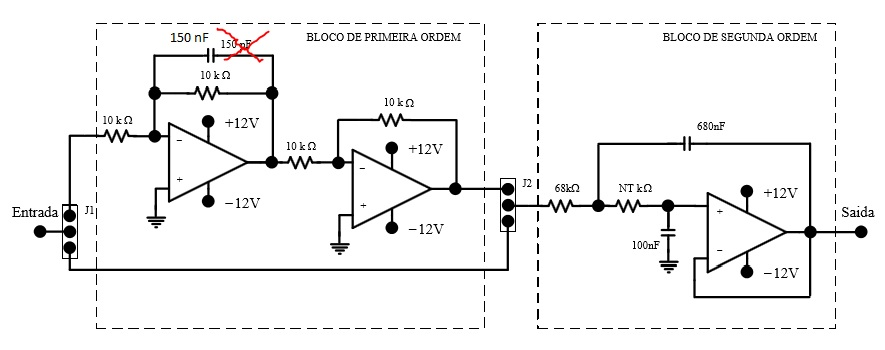
\includegraphics[scale=0.6]{./img/plantaProposta.jpg}
	\label{fig:plantaProposta_1}
	\legend{Fonte: Slide de apresentação do projeto}
\end{figure}

A \autoref{fig:esquematico_1} ilustra o esquemático da planta apresentada na \autoref{fig:plantaProposta_1} em conjunto com o sistema de controle formando um sistema em malha fechada.
A interface do sistema digital com o sistema analógico, no sentido do fluxo de sinal do sistema digital para o analógico, será feito com modulação de largura de pulso (PWM - Pulse Width Modulation). 
A interface no sentido do fluxo de sinal do sistema analógico para o sistema digital será feito por meio de conversores analógicos digitais.

\begin{figure}[htb!]
	\centering
	\caption{Esquemático do Sistema - Planta e Controlador.}
	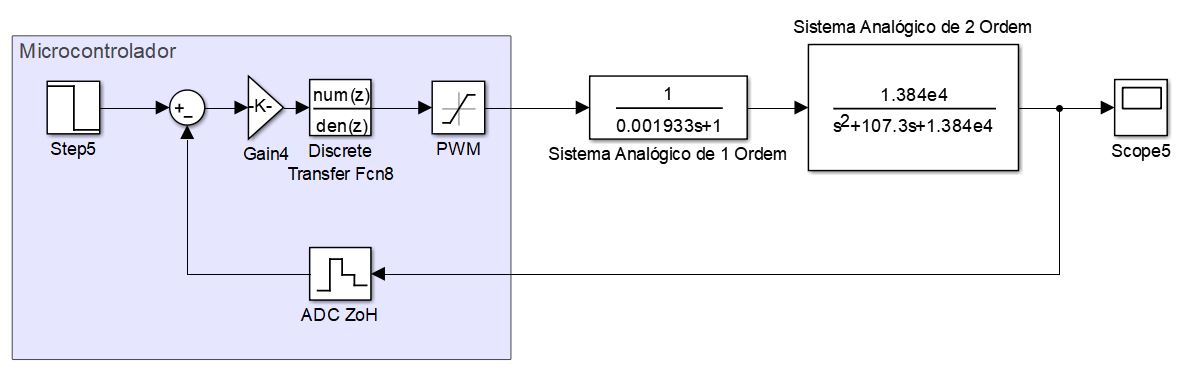
\includegraphics[scale=0.5]{./img/modeloSistemaDeControle_intro.JPG}
	\label{fig:esquematico_1}
	\legend{Software: MATLAB - Simulink}
\end{figure}

\pagebreak



\section{\textbf{Montagem da planta e sistema de controle.}}

\subsection{Montagem da planta em placa de circuito impresso.}
 
O layout da planta foi desenhado por meio do \textit{software} Altium. O amplificador operacional utilizado foi o LM224n. O layout abaixo segue o esquemático da \autoref{fig:plantaProposta_1} com um diodo zener 1N4734A de 5.6 V para proteção do ADC do microcontrolador contra tensão acima das suportadas pelo pino do microcontrolador (que segundo o \textit{datasheet} é 5.5 V para os microcontroladores da Cypress da linha PSOC 5LP).
Essa proteção é pertinente uma vez que os amplificadores operacionais irão operar com tensão simétrica de 12 V. 

\begin{figure}[htb!]
	\centering
	\caption{Layout da placa de circuito impresso.}
	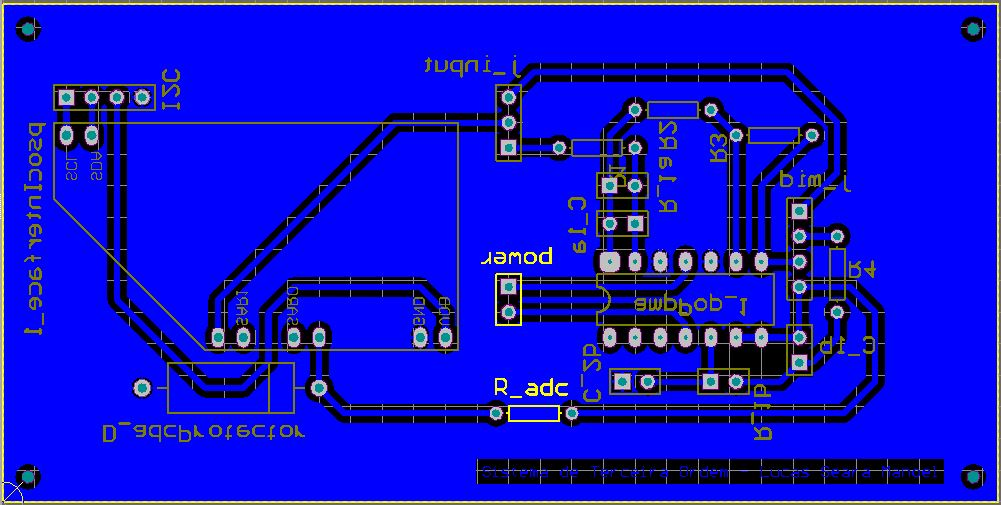
\includegraphics[scale=0.5]{./img/layout.JPG}
	\label{fig:layout}
	\legend{Software: Altium}
\end{figure}

A \autoref{fig:plantaMontagem_4.jpg} apresenta como ficou a placa de circuito impresso após corrosão. As dimensões da placa são 5x10 cm:

\begin{figure}[htb!]
	\centering
	\caption{Placa de circuito impresso após corrosão.}
	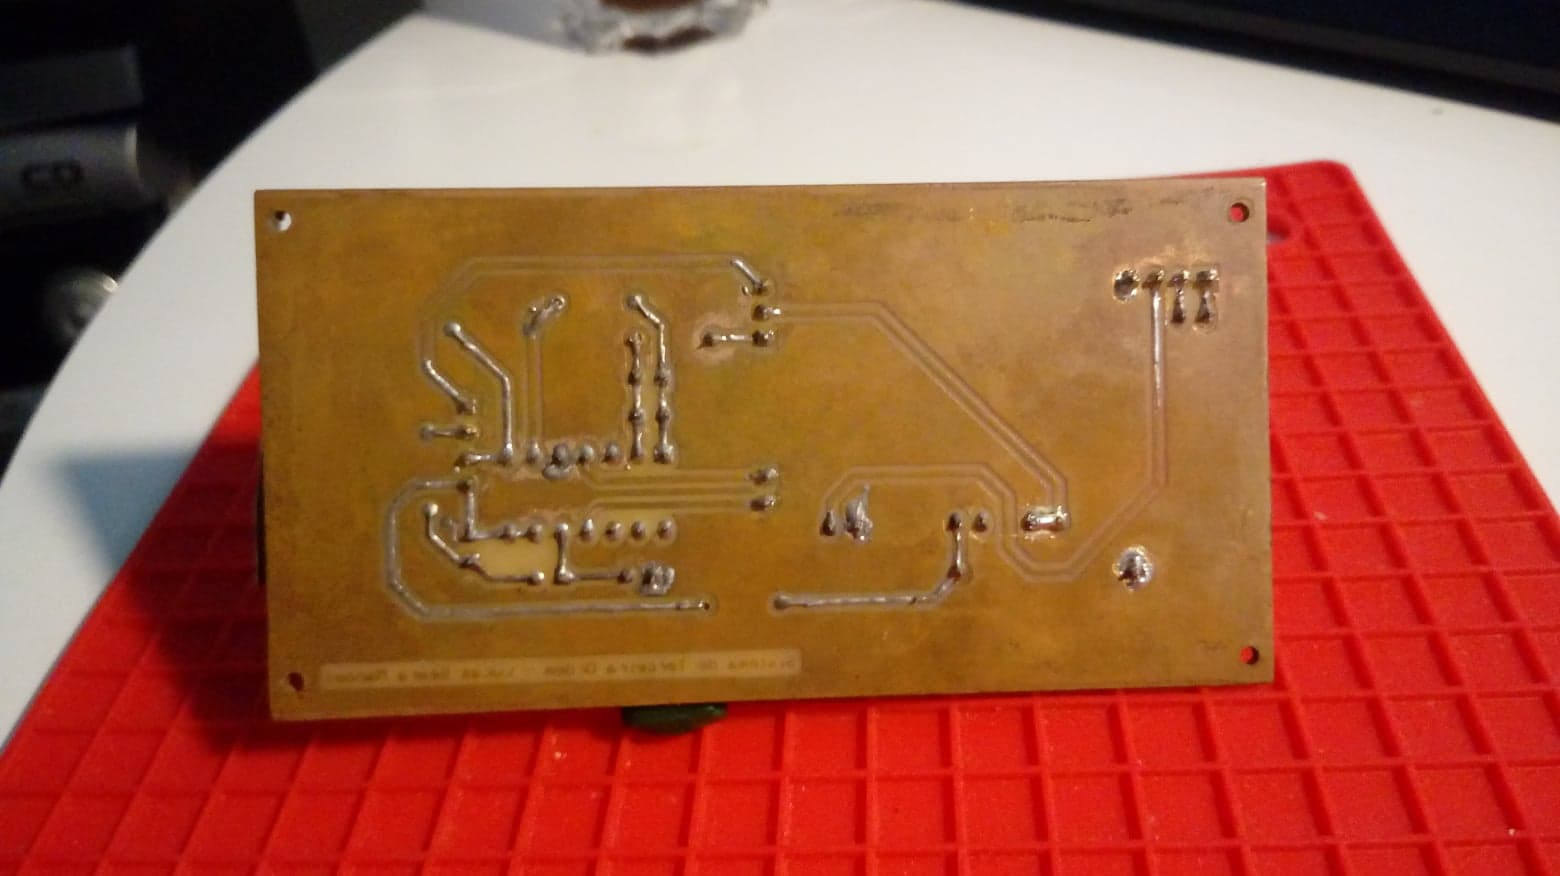
\includegraphics[scale=0.23]{./img/plantaMontagem_4.jpg}
	\label{fig:plantaMontagem_4.jpg}
\end{figure}

\pagebreak

O layout da planta foi desenhado de forma que os elementos chaves que definem as constantes de tempo possam ser facilmente substituídos. 
Dessa forma é evitado que seja preciso reaquecer as trilhas de cobre da placa de fenolite em um processo de retrabalho de soldagem.
Essa abordagem facilitou a troca de um dos capacitores do sistema de primeira ordem que foi substituído durante o decorrer do projeto (essa troca está indicada com uma marcação X em vermelho na \autoref{fig:plantaProposta_1} - troca do capacitor de 150 pF para 150 nF). 

\begin{figure}[htb!]
	\centering
	\caption{Placa de circuito - Top Layer.}
	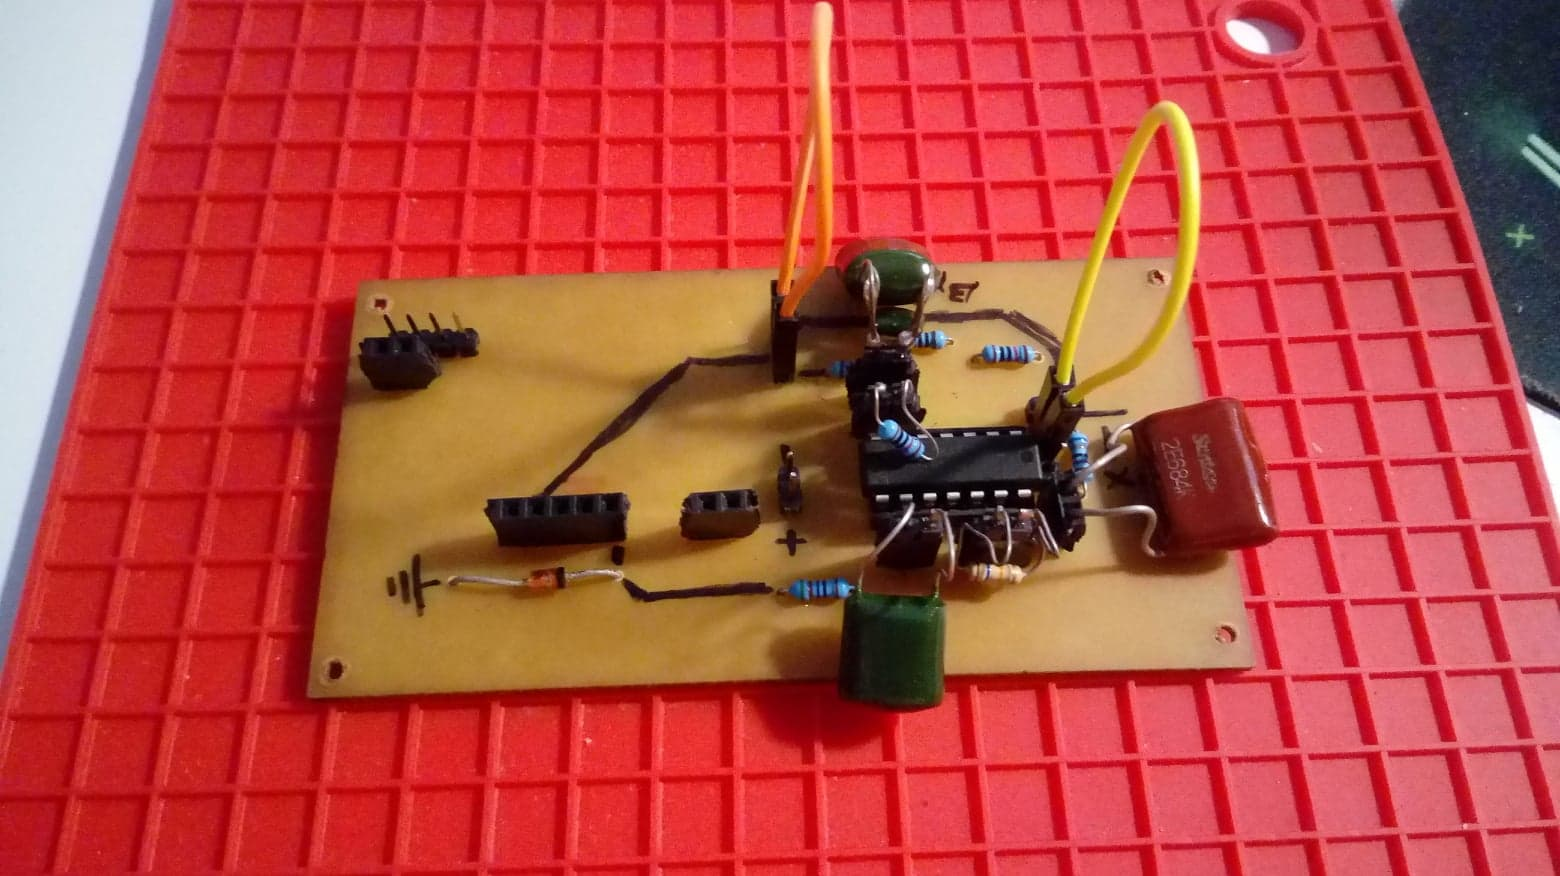
\includegraphics[scale=0.23]{./img/plantaMontagem_2.jpg}
	\label{fig:plantaMontagem_2}
\end{figure}

Para prevenir o mal contato entre os terminais dos componentes removíveis com a planta, foram soldados aos terminais dos componentes pinos que exercem um bom encaixe com os \textit{headers} da planta.
\begin{figure}[htb!]
	\centering
	\caption{Placa de circuito impresso - Componentes Removíveis.}
	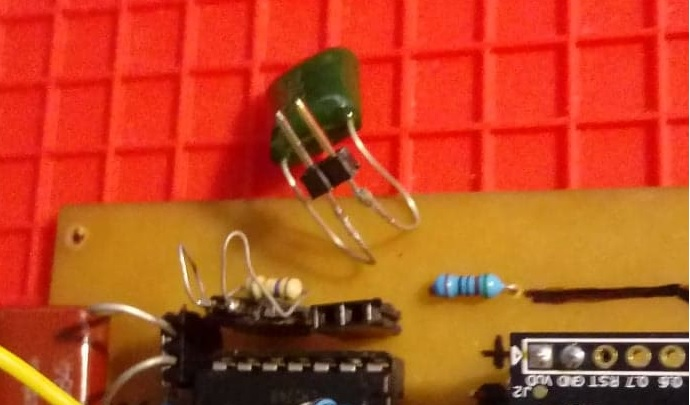
\includegraphics[scale=0.7]{./img/plantaMontagem_3.jpg}
	\label{fig:plantaMontagem_3}
\end{figure}

\pagebreak

\subsection{Implementação do sistema de controle com uso do dispositivo PSOC.}
\label{sec:implement_psoc}
O layout foi desenvolvido com base na placa de desenvolvimento CY8CKIT-059 da Cypress. 
Essa placa de desenvolvimento carrega um PSOC (\textit{Programable System On Chip}) da família CY8C58LP.
O dispositivo presente na placa é o CY8C5888LTI-LP097 que é um dispositivo que carrega um microcontrolador ARM Cortex-M3 em conjunto com periféricos que podem ter suas disposições programadas dentro do componente.

\begin{figure}[htb!]
	\centering
	\caption{Planta com Microcontrolador acoplado.}
	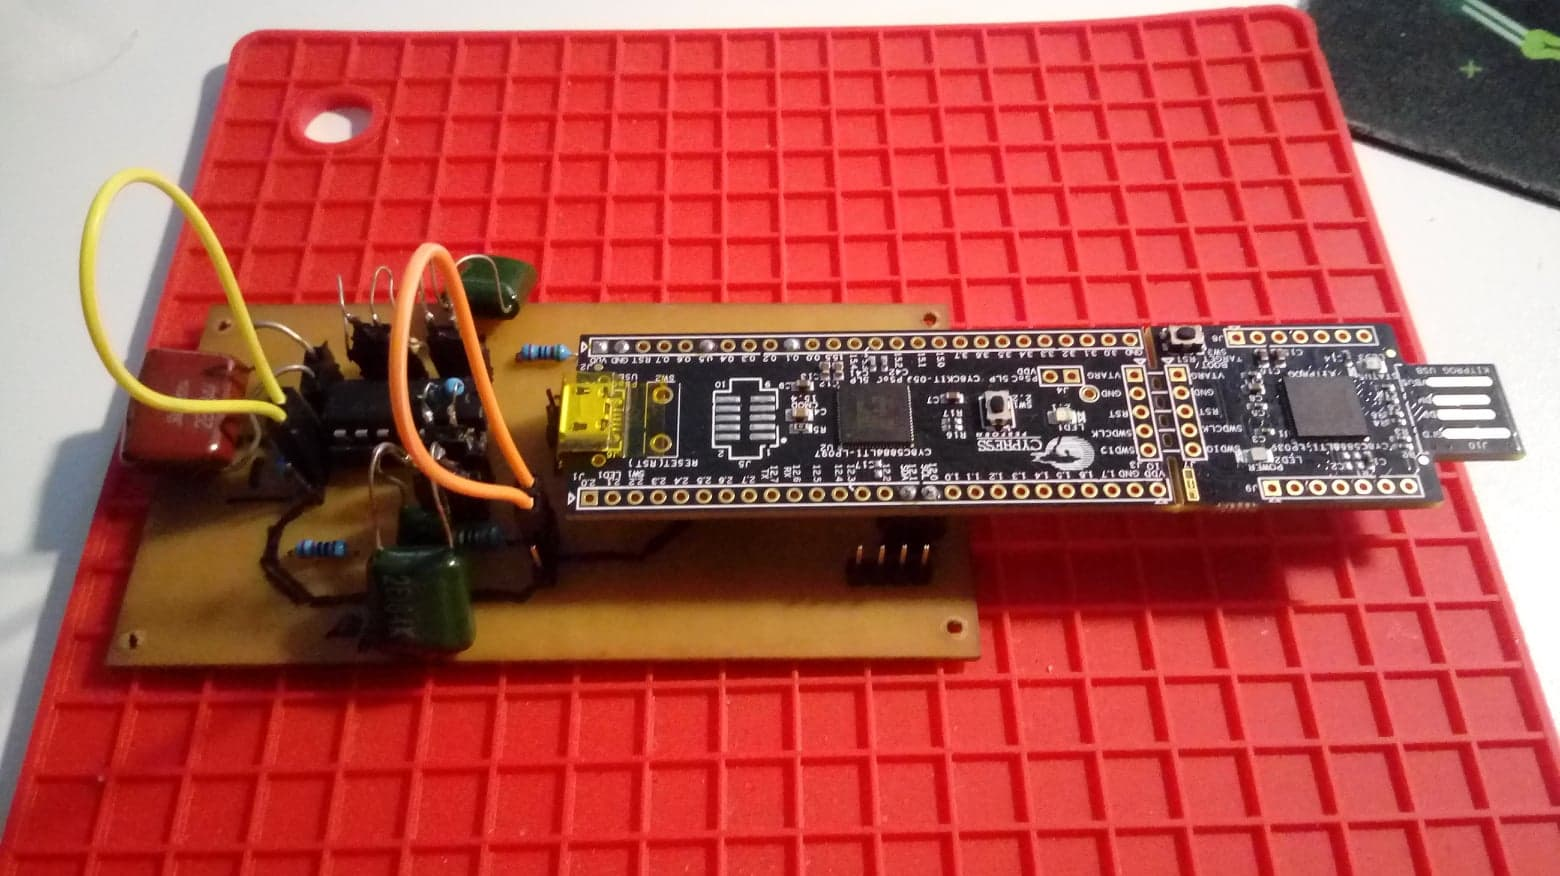
\includegraphics[scale=0.14]{./img/plantaMontagem_1.jpg}
	\label{fig:plantaMontagem_1}
\end{figure}

Esse componente possui vários periféricos disponíveis para uso, incluindo periféricos analógicos como amplificadores operacionais, comparadores, PGAs (amplificadores de ganho programável), TIAs (Amplificadores de Trans-impedância), Mixers e outros. Os principais periféricos utilizados nessa atividade foram o ADC delta sigma de 16 bits e um PWM também de 16 bits.
A \autoref{fig:PSOC5LP_features} retirada do \textit{datasheet} do componente mostra um mapa dos periféricos disponíveis:
\begin{figure}[htb!]
	\centering
	\caption{Mapa dos periféricos do PSOC da família CY8C58LP.}
	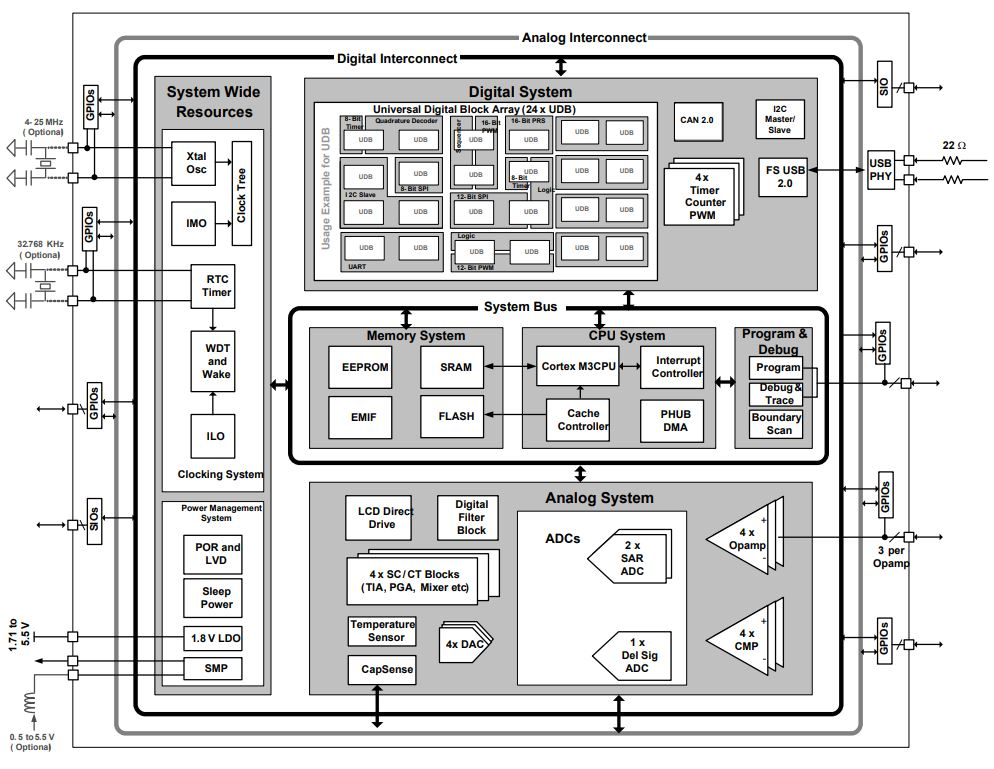
\includegraphics[scale=0.55]{./img/PSOC5LP_features.JPG}
	\label{fig:PSOC5LP_features}
\end{figure}

\pagebreak

A disposição dos periféricos é estabelecida via diagrama de blocos como o esquemático da \autoref{fig:PSOC_esquematico}.
A partir de um sinal de \textit{clock} de 66 MHz, sinais de \textit{clock} de menor frequência serão gerados para que o PWM seja sincronizado ao sinal de interrupção. Com uma série de três contadores de 8 bits seguido de um contador que irar contar até 4, o período de amostragem do sistema será de 3.9719 ms (praticamente 4 ms). 
Periféricos como a interface UART e um TIMER para contagem do tempo de processamento também foram adicionados como pode ser visto na \autoref{fig:PSOC_esquematico}:


\begin{figure}[htb!]
	\centering
	\caption{Mapa dos periféricos do PSOC da família CY8C58LP.}
	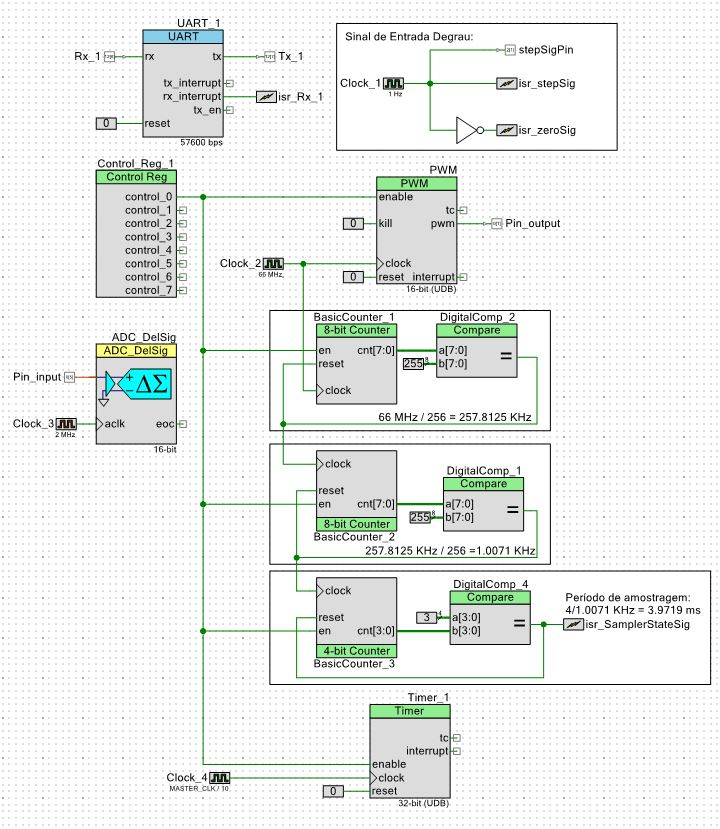
\includegraphics[scale=0.65]{./img/PSOC_esquematico.JPG}
	\label{fig:PSOC_esquematico}
	\legend{Software: PSoC Creator 4.2}
\end{figure}

O dispositivo PSOC irá implementar o hardware descrito na \autoref{fig:PSOC_esquematico} e o núcleo do processador ARM Cortex-M3 irá interagir com esse hardware por meio dos pinos de interrupção iniciados pela sigla isr. 
Logo a cada acionamento do pino de interrupção SamplerStateSig, uma função responsável por processar o sinal lido pelo ADC para atualizar o valor da saída PWM será chamada.
O sinal lido pelo ADC junto ao tempo de processamento contado pelo TIMER também é enviado via UART para que possa ser visualizado no computador.
O código completo do firmware está disponível no \autoref{app:FirmwareCompleto}.

\pagebreak

O periférico conversor digital do tipo delta sigma foi configurado como é mostrado na \autoref{fig:ADCconfig}.
Operando com uma frequência de 1.5 MHz, o periférico está efetuando 5358 leituras por segundo - período de amostragem de 187 $\mu$s. 
Sendo a resolução de 16 bits, o erro de quantização é de $2^{-16} = 0.0015\%$ que corresponde a uma relação sinal ruído de 96 dB.


\begin{figure}[htb!]
	\centering
	\caption{Medição do sobressinal do sistema de segunda ordem.}
	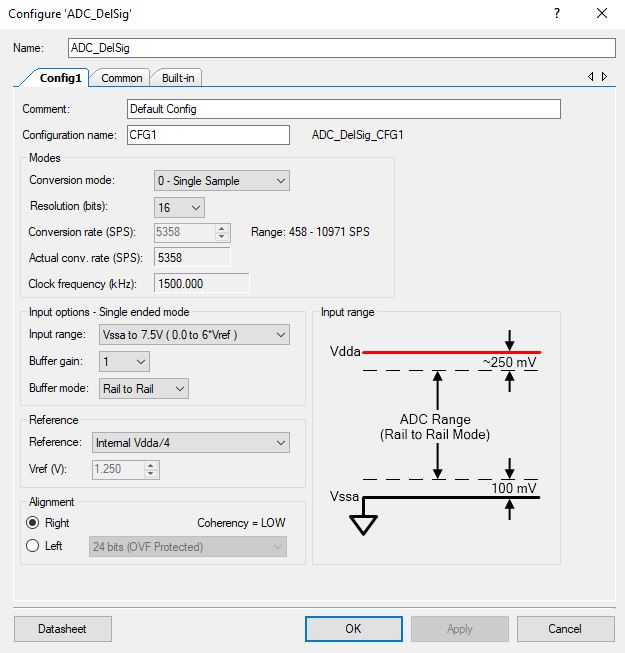
\includegraphics[scale=0.9]{./img/ADCconfig.JPG}
	\label{fig:ADCconfig}
	\legend{Software: PSoC Creator 4.2}
\end{figure}

\pagebreak

Periférico de PWM possui a mesma resolução do ADC utilizado.
Funcionando com um \textit{clock} de 66 MHz, período de um ciclo irá corresponder a 992.97 $\mu$s com um \textit{dutycycle} podendo representar 65536 valores diferentes.
A configuração do periférico de PWM é apresentada na \autoref{fig:PWMconfig}.

\begin{figure}[htb!]
	\centering
	\caption{Configuração do PWM.}
	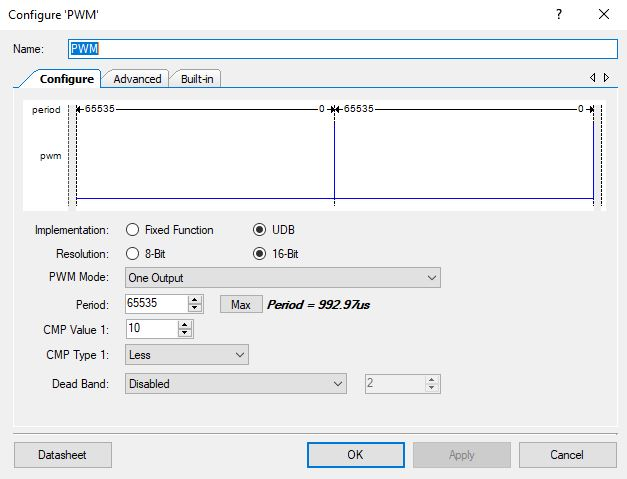
\includegraphics[scale=0.90]{./img/PWMconfig.JPG}
	\label{fig:PWMconfig}
	\legend{Software: PSoC Creator 4.2}
\end{figure}

\pagebreak

\section{\textbf{Análise da Planta.}}

\subsection{Análise teórica da Planta.}

Ao analisar a planta da \autoref{fig:plantaProposta_1} é possível notar que o bloco de segunda ordem é uma topologia conhecida denominada de Sallen-Key \cite{sadiku2013}. 
No caso da planta proposta para a atividade, um filtro Sallen-Key passa baixa.

\begin{figure}[htb!]
	\centering
	\caption{Esquemático do filtro de topologia Sallen-Key.}
	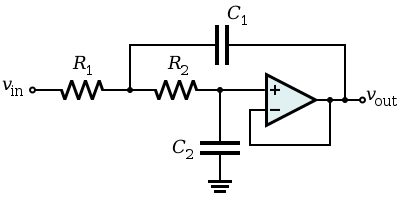
\includegraphics[scale=0.45]{./img/Sallen-Key_Lowpass_General.png}
	\label{fig:Sallen-Key_Lowpass_General}
	\legend{Fonte: Wikipédia}
\end{figure}

A função transferência do filtro Sallen-Key é conhecida e é apresentada abaixo em concordância com a ordem dos componentes da \autoref{fig:Sallen-Key_Lowpass_General}:
$$
	G_{2}(s) = \frac{1}{R_1R_2C_1C_2s^2 + (R_1+R_2)C_2s + 1}
$$

Utilizando os valores da \autoref{fig:plantaProposta_1} (onde NT = 16), a função transferência do sistema de segunda ordem é:

$$
	G_{2}(s) = \frac{1}{7.398*10^{-5}s^2 + 0.0084s + 1}
$$

A \autoref{fig:sallenKey_step} mostra graficamente a resposta ao degrau da função transferência do filtro Sallen-Key. Nessa figura está marcado o tempo de acomodação $T_s (5\%)$ e o valor da amplitude onde ocorre o valor de máximo sobressinal $M_p$:


\begin{figure}[htb!]
	\centering
	\caption{Resposta ao degrau do filtro Sallen-Key.}
	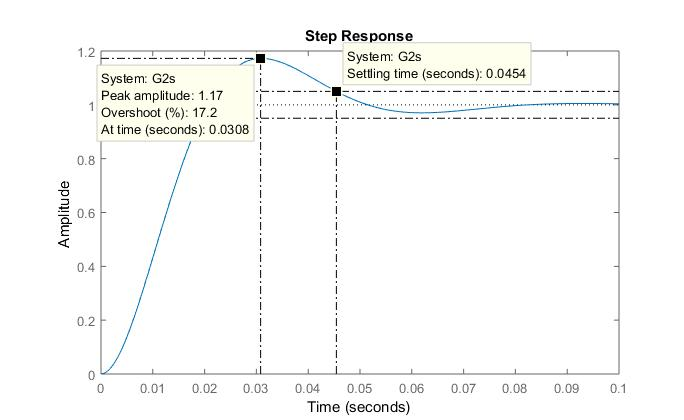
\includegraphics[scale=0.5]{./img/sallenKey_step.JPG}
	\label{fig:sallenKey_step}
	\legend{Software: MATLAB}
\end{figure}

\pagebreak

O primeiro bloco da \autoref{fig:plantaProposta_1} é de simples análise e trata de um sistema de primeira ordem. 
Como a constante de tempo $\tau$ é definida pela multiplicação do valor do resistor com o capacitor do ramo de realimentação: 
$$\tau = RC = 150e-9 * 10e-3 = 1.5 ms.$$
Logo a função transferência do sistema de primeira ordem é:
$$
	G_{1}(s) = \frac{1}{0.0015s + 1}
$$
Ao juntar o sistema de primeira ordem com o sistema de segunda ordem, o sistema resultante assume ordem 3 e a sua função transferência é:
$$
	G(s) = G_{1}(s)*G_{2}(s) = \frac{1}{1.11*10^{-7} s^3 + 8.658*10^{-5} s^2 + 0.0099 s + 1}
$$
A \autoref{fig:sistemaTerceiraOrdem_step} apresenta a resposta ao degrau do sistema de terceira ordem:
\begin{figure}[htb!]
	\centering
	\caption{Resposta ao degrau do sitema completo da planta - Ordem três.}
	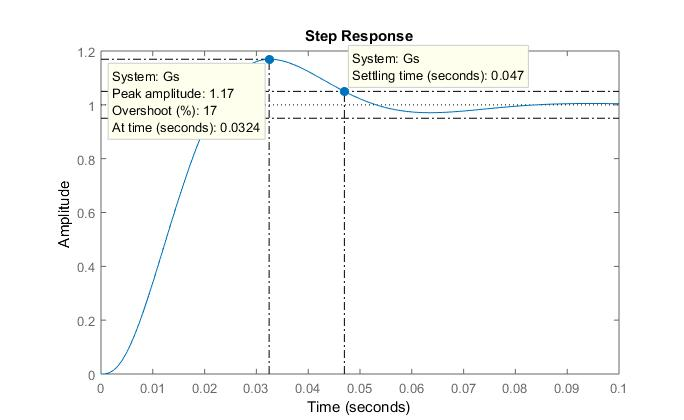
\includegraphics[scale=0.5]{./img/sistemaTerceiraOrdem_step.JPG}
	\label{fig:sistemaTerceiraOrdem_step}
	\legend{Software: MATLAB}
\end{figure}

É possível notar uma semelhança entre o sistema de segunda ordem, $G_{2}$, com o sistema de terceira ordem $G(s)$. Porém vale lembrar que o sistema de terceira ordem, por ter um polo a mais que o sistema de segunda ordem, possui um lugar das raízes diferente e suas características tenderão a serem diferentes com o aumento do ganho de um suposto controlador (em um contexto onde a planta é controlada em malha fechada).
\pagebreak

\subsection{Análise experimental da planta.}

Como ja discutido na análise teórica, o sistema apresentado na \autoref{fig:plantaProposta_1} é composto de dois blocos.
Um primeiro bloco é composto por um sistema de primeira ordem com ganho unitário.
O parâmetro relevante para que esse sistema possa ser modelado na forma de função transferência, por meio de análise experimental, é a sua constante de tempo $\tau$.
Dessa forma a função transferência do sistema de primeira ordem pode ser modelada como:
$$
	G_{1}(s) = \frac{1}{s\tau + 1}
$$

Uma forma de medir o $\tau$ é aplicando um sinal do tipo degrau na entrada do sistema de primeira ordem. E com um osciloscópio é possível medir o tempo que o sinal de resposta leva para acompanhar a entrada. 
No caso da \autoref{fig:3Tau_primeiraOrdem} foi medido quanto tempo a saída do sistema leva para mudar 95\% a sua amplitude. 
Segundo \citeonline{Ogata2014}, a amplitude de um sistema de primeira ordem leva três vezes a contante de tempo $\tau$ para atingir 95\% da amplitude do sinal degrau aplicado como entrada.

\begin{figure}[htb!]
	\centering
	\caption{Medição de três vezes a constante de tempo $\tau$ - 95\% do sinal.}
	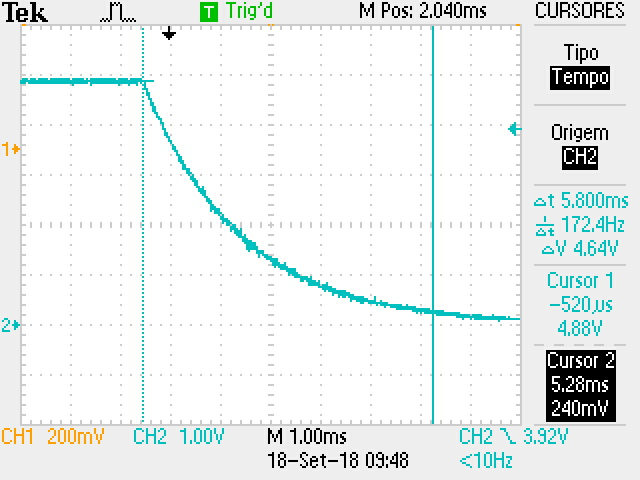
\includegraphics[scale=1.4]{./img/3Tau_primeiraOrdem.JPG}
	\label{fig:3Tau_primeiraOrdem}
	\legend{Osciloscópio Tektronics Tds1002c}
\end{figure}

A \autoref{fig:3Tau_primeiraOrdem} indica que o sistema levou 5.8 ms para atingir 95\% do sinal. 
Logo a constante de tempo é um terço desse valor: $\tau$ = 1.933 ms. 
Dessa forma o sistema de primeira ordem do primeiro bloco pode ser modelado na forma de função transferência como:
$$
	G_{1}(s) = \frac{1}{s0.001933 + 1}
$$

\pagebreak

Para encontrar o modelo matemático de um sistema de segunda ordem com método experimental, duas grandezas são relevantes medir no ensaio de entrada ao degrau: O máximo sobressinal $M_{p}$ e o tempo de pico $T_{p}$.
Com essas duas grandezas é possível encontrar o coeficiente de amortecimento $\zeta$ e frequência natural do sistema $\omega_n$. Com $\zeta$ e $\omega_n$ é possível modelar o sistema na forma de função transferência mostrada abaixo\cite{Ogata2014}:
$$
	G_{2}(s) = \frac{{\omega_n}^2}{s^2 + 2\zeta\omega_ns + {\omega_n}^2}
$$

A \autoref{fig:segundaOrdem_sobreSig} mostra a medição do sobressinal $M_{p}$. Da forma que é possível constatar que o máximo sobressinal para um degrau de amplitude de 500mV é 100 mV.

\begin{figure}[htb!]
	\centering
	\caption{Medição do sobressinal do sistema de segunda ordem.}
	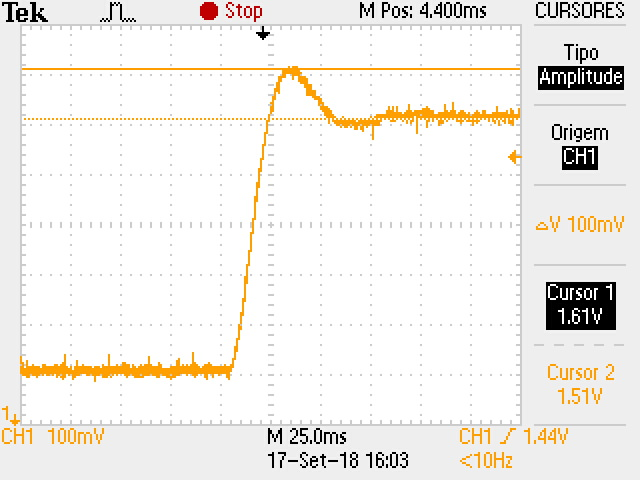
\includegraphics[scale=1.4]{./img/segundaOrdem_sobreSig.JPG}
	\label{fig:segundaOrdem_sobreSig}
	\legend{Osciloscópio Tektronics Tds1002c}
\end{figure}

O valor $M_{p}$ é definido como o porcentual da amplitude do sinal degrau aplicado na entrada. Logo 100 mV representa 20\% de 500mV. Assim o valor de sobressinal pode ser definido como $M_{p}$ = 0.2. 
A literatura de \citeonline{Ogata2014} indica que $M_{p}$ se relaciona com $\zeta$ como:

$$
	M_{p} = e^{-\frac{\zeta}{\sqrt{1-\zeta^2}}\pi}
$$

A equação acima pode ser resolvida numericamente com auxílio do computador. Dessa forma, utilizando os valores medidos, o valor de $\zeta$ (zeta) calculado numericamente apresenta o resultado:

$$
	\zeta = 0.4559
$$

\pagebreak

A segunda grandeza para que o sistema de segunda ordem possa ser modelado em forma de função transferência é o tempo de pico $T_{p}$ da sua resposta ao degrau. A \autoref{fig:segundaOrdem_Tp} mostra a medição do tempo de pico como sendo $T_{p}$ = 30 ms.

\begin{figure}[htb!]
	\centering
	\caption{Medição do tempo de pico do sistema de segunda ordem.}
	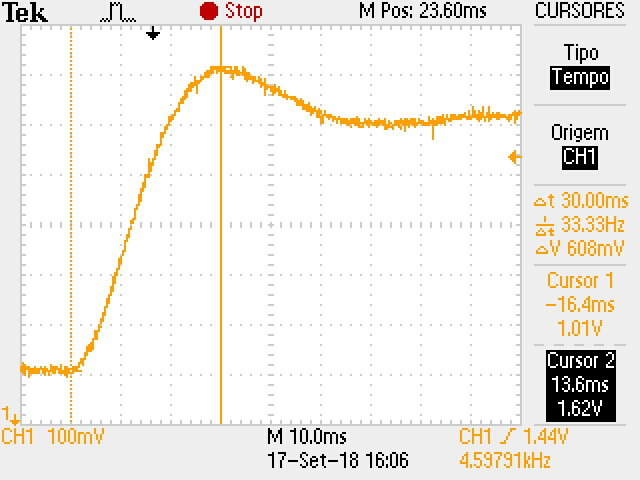
\includegraphics[scale=1.4]{./img/segundaOrdem_Tp.JPG}
	\label{fig:segundaOrdem_Tp}
	\legend{Osciloscópio Tektronics Tds1002c}
\end{figure}

Conhecendo o $\zeta$ anteriormente calculado e o tempo de pico $T_{p}$, a frequência natural do sistema $\omega_n$ se relaciona com essas grandezas por meio da equação \cite{Ogata2014}:

$$
	\omega_n = -\frac{\pi}{T_{p}\sqrt{1-\zeta^2}} = -\frac{\pi}{0.03\sqrt{1-0.4559^2}} = 117.66
$$
Com os valores de $\zeta$ = 0.4559 r $\omega_n$ = 117.66 definidos, a os coeficientes da equação de transferência do sistema de segunda ordem são definidos como:
$$
	G_{2}(s) = \frac{{\omega_n}^2}{s^2 + 2\zeta\omega_ns + {\omega_n}^2} = \frac{13840}{s^2 + 107.3s + 13840}
$$
E o sistema resultante é:
$$
	G(s) = G_{1}(s)*G_{2}(s) = \frac{1}{1.4*10^{-7} s^3 + 8.721*10^{-5} s^2 + 0.0097 s + 1}
$$

\pagebreak

\subsection{Comparação entre modelo teórico e experimental da planta.}

As funções transferências modeladas de forma teórico e experimental se apresentaram muito parecidas.

Teórico:
$$
	G(s) = \frac{1}{1.11*10^{-7} s^3 + 8.658*10^{-5} s^2 + 0.0099 s + 1}
$$

Experimental:
$$
	G(s) = \frac{1}{1.4*10^{-7} s^3 + 8.721*10^{-5} s^2 + 0.0097 s + 1}
$$

Isso é comprovado plotando a resposta ao degrau de ambas as funções transferências como apresentado na \autoref{fig:sistemaTerceiraOrdemComp_step}.
A curva vermelha, com maior valor de $M_p$, representa a resposta ao degrau da função transferência obtida de forma experimental e a curva azul representa a função transferência obtida de forma teórica.
Uma pequena diferença surge pois a curva obtida de forma teórica não leva em conta as não idealidades dos componentes, principalmente dos amplificadores operacionais.
\begin{figure}[htb!]
	\centering
	\caption{Medição do tempo de pico do sistema de terceira ordem.}
	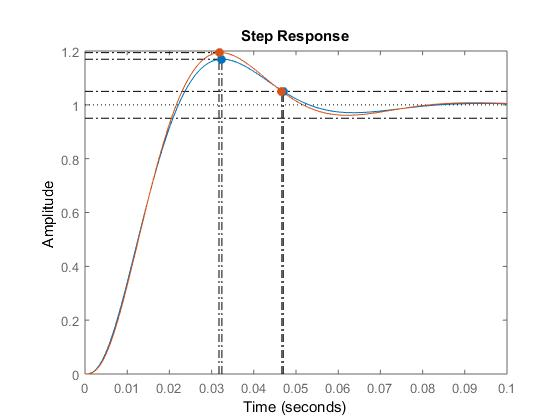
\includegraphics[scale=0.8]{./img/sistemaTerceiraOrdemComp_step.JPG}
	\label{fig:sistemaTerceiraOrdemComp_step}
	\legend{Software: MATLAB}
\end{figure}

\pagebreak

Fazendo a medição experimental da resposta ao degrau da planta é possível ver que as funções transferências obtidas se assemelham com a realidade (comparando a \autoref{fig:sistemaTerceiraOrdemComp_step} com a \autoref{fig:tp_terceiraOrdem}).
É possível constatar que ambas as respostas ao degrau possuem um tempo de máximo sobressinal de $T_p$ = 33 ms e um valor de sobressinal próximo a $M_p$ = 0.2.
\begin{figure}[htb!]
	\centering
	\caption{Medição do tempo de pico do sistema de ordem 3.}
	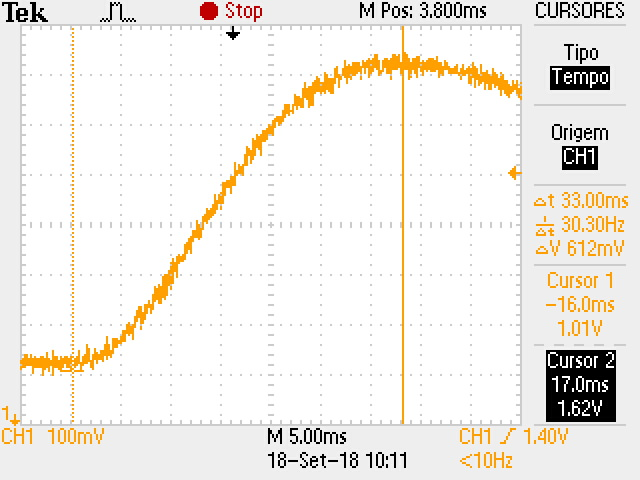
\includegraphics[scale=1.4]{./img/tp_terceiraOrdem.JPG}
	\label{fig:tp_terceiraOrdem}
	\legend{Osciloscópio Tektronics Tds1002c}
\end{figure}

O modelo escolhido como representação da planta foi o modelo experimental pois esse retrata de forma mais realista a planta a ser controlada. Pois leva em conta as reatâncias intrínsecas dos componentes que não são consideradas numa análise teórica que considera componentes ideias.

$$
	G(s) = \frac{1}{1.4*10^{-7} s^3 + 8.721*10^{-5} s^2 + 0.0097 s + 1}
$$

\pagebreak

\subsection{Discretização do modelo de tempo contínuo da planta.}

Como o microcontrolador não é capaz de processar sinais de tempo contínuo, um modelo de tempo discreto da planta precisa ser estabelecido.
Como o sistema apresenta resposta subamortecida e considerando a frequência natural do sistema de terceira ordem com valor aproximado a frequência natural do bloco de segunda ordem de valor $\omega_n = 117.66$, a literatura recomenta a utilização de uma taxa de amostragem de oito a dez vezes maior que $\omega_n$ da resposta do sinal após a compensação\cite{Ogata_DTC_1995}.
Como o requisito do projeto é diminuir o  tempo de acomodação $T_s$ e sobressinal $M_p$ pela metade, a frequência natural deve ser dobrada assumindo o valor $\omega_n = 2*117.66 = 235.32$ e o o fator de amortecimento $\zeta$ deve corresponder a um sobressinal de 0.1, logo $\zeta = 0.6$.
Assim a frequência de amostragem pode ser definida como (considerando $\zeta=0.6$ e $\omega_n = 235.32$):
$$
	f_s = 10 * \frac{\omega_n\sqrt{1-\zeta^2}}{2\pi} \simeq 250 Hz
$$
Com o valor de $f_s$ estabelecido, consequentemente o período de amostragem: $$T=\frac{1}{f_s} = 4 ms \simeq 4 * 0.99297 ms$$
O sistema \textit{Sample-Hold} de ordem zero é definido como:
$$Zoh(s)=\frac{1-e^{-Ts}}{s} = \frac{1-e^{-0.004s}}{s}$$
Logo a função transferência da planta discretizada pode ser definida como
$$G(z)=\mathscr{Z}\{Zoh(s)*G(s)\}=(1-z^{-1})\mathscr{Z}\{\frac{G(s)}{s}\}$$
Assumindo $T = 4 * 0.99297 ms$ devido a base de tempo de 66 MHz utilizada no microcontrolador (\autoref{sec:implement_psoc}):
$$G(z) =\frac{0.04241z^2 + 0.09738z + 0.01247}{z^3 - 1.607z^2 + 0.8424z - 0.08366}=\frac{0.042406(z+2.16)(z+0.1361)}{(z-0.1281)(z^2 - 1.478z + 0.653)}$$
A resposta ao degrau da planta discretizada está apresentada na \autoref{fig:sistemaDricretizado_step}.

\begin{figure}[htb!]
	\centering
	\caption{Resposta ao degrau do planta discretizada.}
	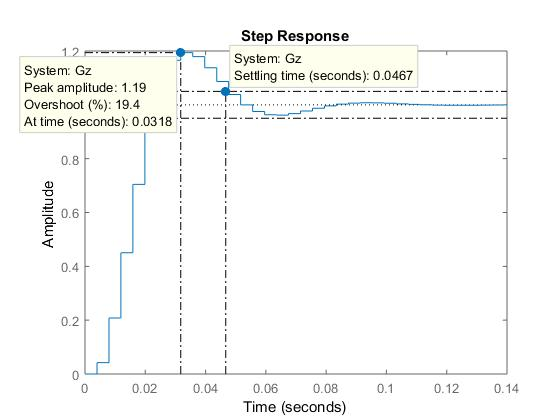
\includegraphics[scale=0.46]{./img/sistemaDricretizado_step.JPG}
	\label{fig:sistemaDricretizado_step}
	\legend{Software: MATLAB}
\end{figure}

\pagebreak

Por meia da interface UART é possível verificar a leitura do ADC para comparação da resposta á entrada degrau unitário apresentada na \autoref{fig:sistemaDricretizado_step} com a leitura discretizada que o ADC faz da planta. 
Na \autoref{fig:stepPlanta_microCtrl} é possível verificar uma semelhança bem grande entre a simulação e a realidade.
É possível notar o mesmo número de amostras entre o inicio da resposta e o tempo de pico: $T_p/T=8$ amostras.
Também é possível verificar o sobre sinal considerando que:
$$
	100\% => 0.500
$$
$$
	M_p\% + 100\%=> 1.587 - 0.998 = 0.589 => 117.8\%
$$
$$
	M_p\% = 17.8\%
$$
Tempo de acomodação de acomodação $T_s (5\%)$ medido foi $(145 - 133)*T = 12*T = 12*(4*0.9929 ms)= 47.7 ms$, que é bem próximo ao valor da simulação apresentado na \autoref{fig:sistemaDricretizado_step}, que é $46.7 ms$.

\begin{figure}[htb!]
	\centering
	\caption{Resposta ao degrau do planta discretizada.}
	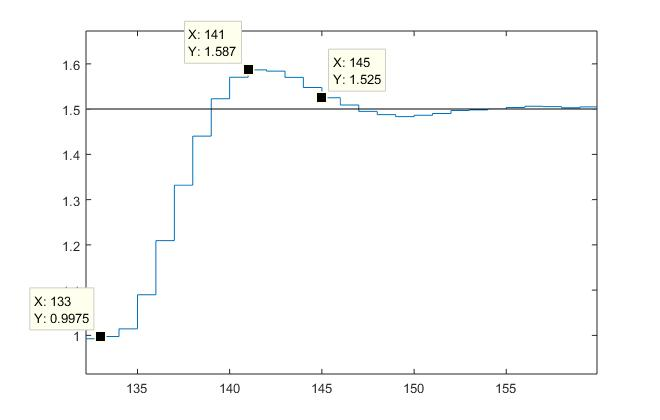
\includegraphics[scale=0.7]{./img/stepPlanta_microCtrl.JPG}
	\label{fig:stepPlanta_microCtrl}
	\legend{Software: MATLAB}
\end{figure}

\pagebreak

\subsection{Análise de erro de regime permanente}

Fazendo um teste por meio do teorema do valor final, uma propriedade da transformada Z que pode ser verificada na literatura de \citeonline{lathi2014}, considerando que Gz será a função transferência de malha aberta (FTMA), foi verificado um erro á entrada degrau unitário.
$$K_p = \lim_{z\to1} FTMA(z) = \lim_{z\to1} G(z) = 1$$ 
$$e(\infty) = \frac{1}{1+K_p} = 0.5$$

\begin{figure}[htb!]
	\centering
	\caption{Verificação do erro ao degrau da $FTMF(z)$ de $G(z)$.}
	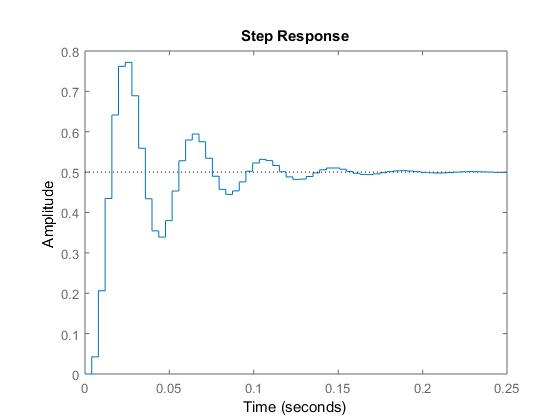
\includegraphics[scale=0.6]{./img/stepErroKp.jpg}
	\label{fig:stepErroKp}
	\legend{Software: MATLAB}
\end{figure}

O acréscimo de um integrador na $FTMA(z)$ faz com que um sistema que é do tipo 0, que apresenta erro á degrau unitário, se torne do tipo 1 não apresentando erro á entrada degrau unitário \cite{Ogata_DTC_1995}(ou fazendo com que o erro tenda a zero como demostrado abaixo).

$$K_p = \lim_{z\to1} \frac{1}{z-1}Gz(z) => \frac{G(z)}{0} = \infty$$ 
$$e(\infty) = \frac{1}{1+K_p} => \frac{1}{1+\infty} = 0$$

\pagebreak

Porém após a aplicação do integrador na $FTMA(z)$ foi verificado que o sistema se tornou instável quando a malha de realimentação foi fechada. 
Isso pode ser verificado no mapa dos polos da $FTMF(z)$ na \autoref{fig:zmapFTMF_1} onde é possível ver que há polos fora do círculo unitário.
Para sistemas de tempo discreto isso indica instabilidade \cite{lathi2014}.

\begin{figure}[htb!]
	\centering
	\caption{Plano Z da malha fechada da planta com integrador.}
	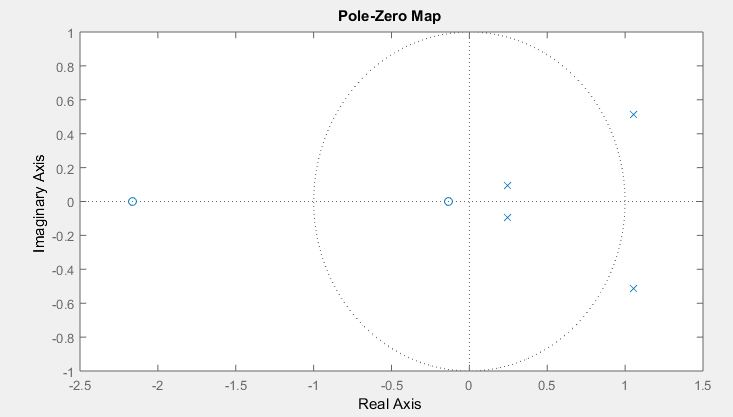
\includegraphics[scale=0.8]{./img/zmapFTMF_1.JPG}
	\label{fig:zmapFTMF_1}
	\legend{Software: MATLAB}
\end{figure}

\pagebreak

Fazendo uma análise do lugar das raízes por meio da $FTMA(z)$, é possível verificar na \autoref{fig:rlocus_1} que um valor muito baixo de ganho é necessário para deslocar os polos da função transferência de malha fechada ($FTMF(z)$) para fora do círculo unitário.

\begin{figure}[htb!]
	\centering
	\caption{Lugar das raizes da planta com integrador.}
	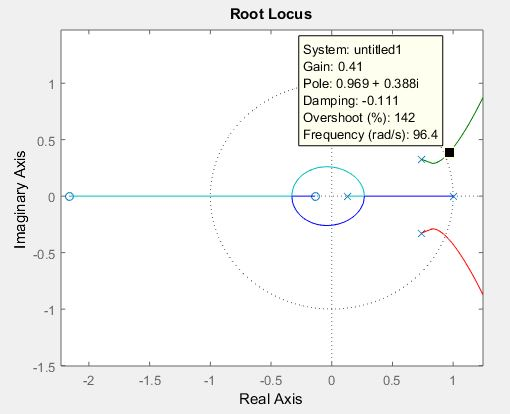
\includegraphics[scale=0.85]{./img/rlocus_1.JPG}
	\label{fig:rlocus_1}
	\legend{Software: MATLAB}
\end{figure}

Uma possibilidade para evitar o deslocamento dos polos complexos para fora do circulo unitário, como mostrado na \autoref{fig:rlocus_2} é a anulação desses com um par complexo conjugado de zeros com o mesmo valor dos polos complexos conjugados presentes na planta.

\begin{figure}[htb!]
	\centering
	\caption{Lugar das raizes da planta com polos anulados.}
	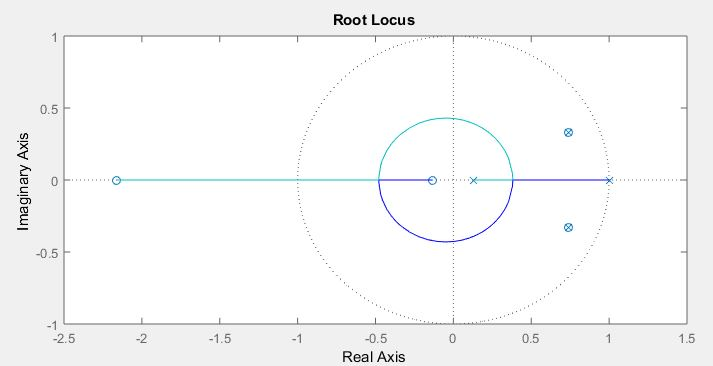
\includegraphics[scale=0.7]{./img/rlocus_2.JPG}
	\label{fig:rlocus_2}
	\legend{Software: MATLAB}
\end{figure}

\pagebreak

O integrador e o par de zeros complexos conjugados precisam ser implementados dentro do microcontrolador para que possam ser estabelecer em série com a planta.
Porém como foram adicionados mais zeros do que polos, uma função transferência com esses elementos acaba tendo a ordem do numerador maior que a do denominador. 
Um sistema assim se tonar não realizável pois é um sistema não causal \cite{lathi2014}. 
$$P1(z)=\frac{1}{z-1}$$
$$Z(z)=z^2 - 1.478 z + 0.6531$$
$$P1(z)*Z(z)=\frac{Y(z)}{X(z)}=\frac{z^2 - 1.478 z + 0.6531}{z-1}$$
$$Y(z)(z-1)=X(z)(z^2 - 1.478 z + 0.6531)$$
$$y[n+1]-y[n]=x[n+2] - 1.478x[n+1] + 0.6531x[n]$$
$$y[n]=x[n+1] - 1.478x[n] + 0.6531x[n-1]+y[n-1]$$
O acréscimo de um polo na origem é suficiente para tonar o sistema causal:
$$P2(z)=\frac{1}{z}$$
$$P1(z)*P2(z)*Z(z)=\frac{Y(z)}{X(z)}=\frac{z^2 - 1.478 z + 0.6531}{z^2-z}$$
$$Y(z)(z^2-z)=X(z)(z^2 - 1.478 z + 0.6531)$$
$$y[n+2]-y[n+1]=x[n+2] - 1.478x[n+1] + 0.6531x[n]$$
$$y[n]=x[n] - 1.478x[n-1] + 0.6531x[n-2]+y[n-1]$$
Porém agora com um polo adicionado na origem o sistema em malha fechada pode se tornar instável com um ganho no ramo direto de aproximadamente igual ou superior a 8.5 (\autoref{fig:rlocus_3}). 

\begin{figure}[htb!]
	\centering
	\caption{Lugar das raizes da planta com polos anulados e polo na origem.}
	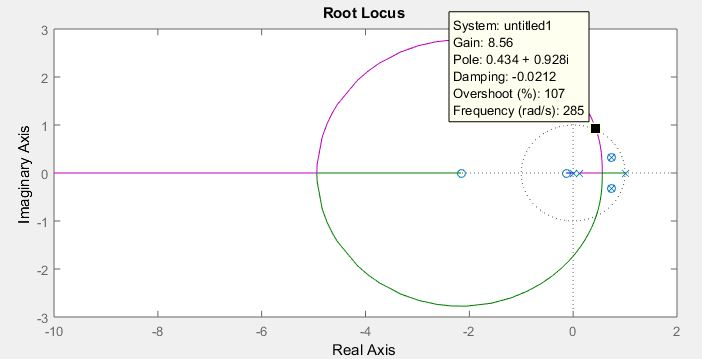
\includegraphics[scale=0.8]{./img/rlocus_3.JPG}
	\label{fig:rlocus_3}
	\legend{Software: MATLAB}
\end{figure}

\pagebreak

Após a aplicação dos zeros complexos conjugados com o integrador e polo na origem, o sistema se tornou estável e sem erro ao degrau unitário. 
A \autoref{fig:stepErroKp_corrigido} mostra a resposta ao degrau da $FTMF(z)$ de $G(z)$ com zeros complexos, integrador e polo na origem.

$$K_p = \lim_{z\to1} G(z)*P1(z)*P2(z)*Z(z) = \lim_{z\to1} \frac{1}{z-1}G(z)*P2(z)*Z(z) => \frac{G(z)*P2(z)*Z(z)}{0} = \infty$$ 
$$e(\infty) = \frac{1}{1+K_p} => \frac{1}{1+\infty} = 0$$

\begin{figure}[htb!]
	\centering
	\caption{Verificação do erro ao degrau da $FTMF(z)$ de $G(z)*P1(z)*P2(z)*Z(z)$.}
	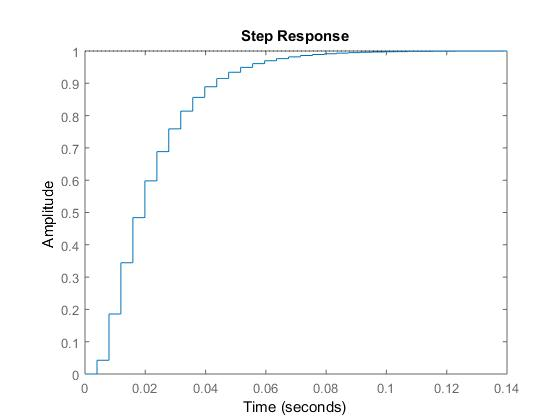
\includegraphics[scale=0.7]{./img/stepErroKp_corrigido.jpg}
	\label{fig:stepErroKp_corrigido}
	\legend{Software: MATLAB}
\end{figure}

\pagebreak

\section{\textbf{Projeto do compensador utilizando o lugar das raizes.}}

Para se obter metade do tempo de acomodação de $5\%$ e sobressinal, é necessário os valores de $T_s/T = 23.5/4 = 5.875$ e um $M_p = 10\%$ (uma vez que os valores medidos da planta são $T_s = 47 ms$ e um $M_p = 20\%$). 
Para atender os requisitos de projeto é verificado que o polo dominante estará dentro da área verde apontada na \autoref{fig:zMap_wn_Zeta}.

\begin{figure}[htb!]
	\centering
	\caption{Mapa das grandezas $\zeta$ e $\omega_n$ no plano Z.}
	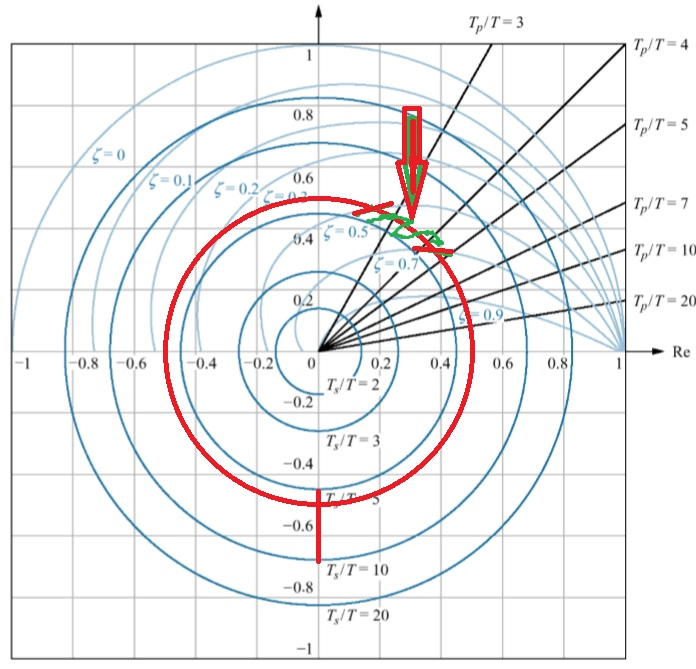
\includegraphics[scale=0.7]{./img/zMap_wn_Zeta.JPG}
	\label{fig:zMap_wn_Zeta}
	\legend{Fonte: Nise, N. - Engenharia de Sistemas de Controle}
\end{figure}

\pagebreak

Com base na literatura de \citeonline{Ogata_DTC_1995}, abaixo é definido a posição do polo dominante que corresponda a um $T_s/T = 5.875$ e $\zeta = 0.6$:

$$\omega_n=\frac{3}{\zeta t_{s5\%}}=\frac{3}{0.6*5.875*T}=214.2723$$
$$\omega_d=\omega_n\sqrt{1-\zeta^2}=171.4178$$
$$|z1|=e^{-T \zeta w_n}=0.6001$$
$$\theta_{z1}=T\omega_n\sqrt{1-\zeta^2}=0.6809$$
$$z1=|z1|e^{i\theta_{z1}}=0.6001e^{i0.6809}=0.4663+i0.3777$$

\begin{figure}[htb!]
	\centering
	\caption{Localização do polo referente as grandezas $\zeta$ e $\omega_n$ no plano Z.}
	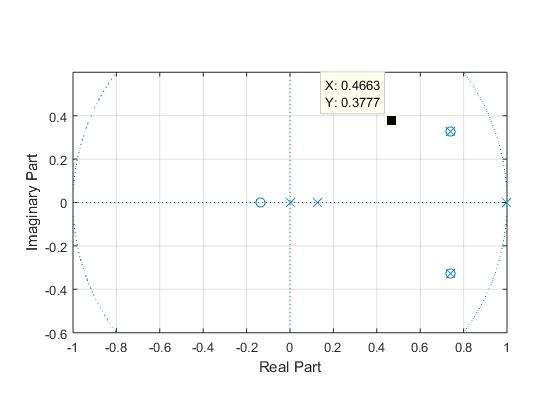
\includegraphics[scale=0.8]{./img/poloDominante.JPG}
	\label{fig:poloDominante}
	\legend{Software: MATLAB}
\end{figure}

\pagebreak

Com a posição do polo dominante definida, o script MATLAB apresentado no \autoref{app:scriptCalcAng} calcula a soma de todos os ângulos dos zeros e polos em relação ao polo dominante.
Para que esse polo seja lugar das raízes, o ângulo resultante desse somatório deve ser $180\degree$ \cite{Ogata_DTC_1995}.
O somatório de todos os ângulos em relação ao polo dominante resulta em $-191.5417\degree$ .
Logo faltam: 

$$180\degree  - 191.5417\degree  = - 11.5417\degree $$

O compensador deve acrescentar $11.5417\degree$.
Logo o compensador a ser projetado é um compensador em atraso pois o polo $\beta$ acontece antes do zero $\alpha$ para que o ângulo fornecido pelo compensador seja positivo \cite{villaca2014}. Como apresentado na \autoref{fig:alphaAndBeta_compensador} o polo e o zero do compensador foram posicionados afim de fornecer $11.5417\degree$:

\begin{figure}[htb!]
	\centering
	\caption{Definição da localização do zero $\alpha$ e polo $\beta$.}
	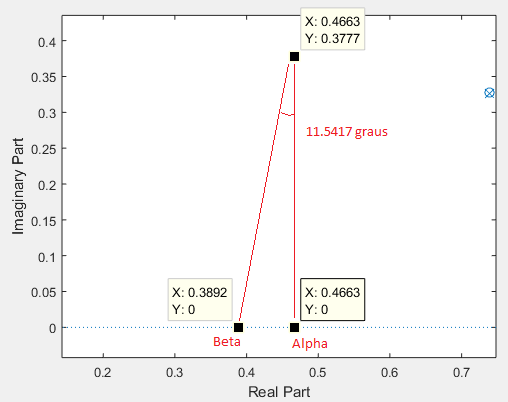
\includegraphics[scale=0.9]{./img/alphaAndBeta_compensador.png}
	\label{fig:alphaAndBeta_compensador}
	\legend{Software: MATLAB}
\end{figure}

$$
	C(z) = K_c * \frac{z - \alpha}{z - \beta} = K_c * \frac{z - 0.4663}{z - 0.3892} 
$$

\pagebreak

Trançando o lugar das raízes da planta, \autoref{fig:rlocus_compensado}, com o compensador é possível ver que o polo dominante é lugar das raízes:

\begin{figure}[htb!]
	\centering
	\caption{Lugar das raízes com o compensador em atraso.}
	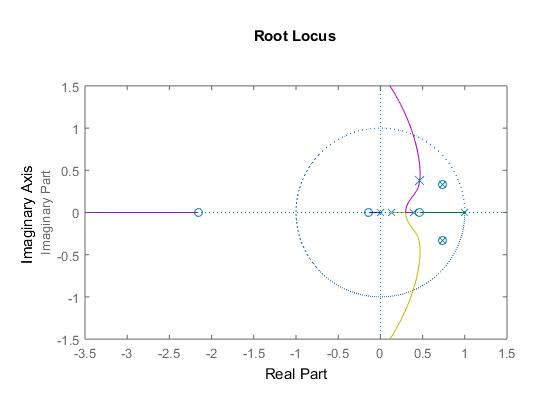
\includegraphics[scale=0.8]{./img/rlocus_compensado.JPG}
	\label{fig:rlocus_compensado}
	\legend{Software: MATLAB}
\end{figure}

Para encontrar o ganho necessário para que o polo dominante seja um dos polos da $FTMF(z)$ da planta compensada, é necessário avaliar o valor de $K_c$ substituindo o valor de z na $FTMA(z)$ pelo valor do polo dominante.
Como o lugar das raízes é baseado na condição de ângulo da $FTMA(z)$ de $180\degree$ e módulo igual a 1 \cite{Ogata2014}:

$$
	C(z) = K_c * \frac{z - \alpha}{z - \beta} = K_c * \frac{z - 0.4663}{z - 0.3892} 
$$

$$
|K_c*\frac{C(z)}{K_c}*G(z)*P1(z)*P2(z)*Z(z)|=1
$$

$$
    K_c  = \left. |\frac{1}{\frac{C(z)}{K_c}*G(z)*P1(z)*P2(z)*Z(z)}| \right\rvert_{z = 0.4663+i0.3777}  = 2.5389
$$
Assim todos os termos da equação de transferência do compensador foram estabelecidos:
$$
	C(z) = K_c * \frac{z - 0.4663}{z - 0.3892}  = 2.5389 * \frac{z - 0.4663}{z - 0.3892}  
$$

\pagebreak

A função transferência do compensador em conjunto com o par de zeros complexos polos, z=0 e z=-1:
$$
    C(z)*Sys(z) = C(z)*P_1(z)∗P_2(z)∗Z_1(z) =2.5389 * \frac{z - 0.4663}{z - 0.3892} *\frac{z^2 - 1.478z + 0.6531}{z^2 - z}
$$
Se colocados em série com a planta, a resposta ao degrau da $FTMF(z)$ é apresentada na \autoref{fig:stepComp}.
$$
    G(z) =\frac{0.04241z^2 + 0.09738z + 0.01247}{z^3 - 1.607z^2 + 0.8424z - 0.08366}
$$
$$
    FTMA(z) = G(z)*C(z)*Sys(z) =2.5389 * \frac{z - 0.4663}{z - 0.3892} *\frac{z^2 - 1.478z + 0.6531}{z^2 - z}*G(z)
$$
$$
    FTMF(z) = \frac{FTMA(z)}{1 + FTMA(z)}
$$

\begin{figure}[htb!]
	\centering
	\caption{Resposta ao degrau da planta em malha fechada após compensação.}
	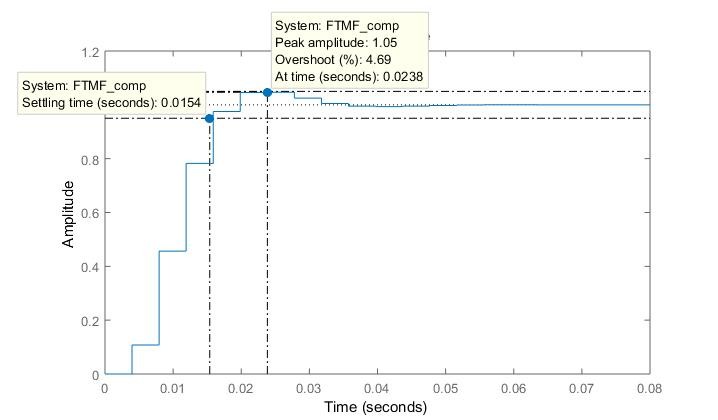
\includegraphics[scale=0.6]{./img/stepComp.JPG}
	\label{fig:stepComp}
	\legend{Software: MATLAB}
\end{figure}

Analisando a \autoref{fig:stepComp} é possível medir um $T_s/T = 3.85$, $M_p = 4.69\%$ e um $T_p/T = 6$. 
Lembrando que os requisitos de projeto são $T_s/T = 5.875$ e $M_p = 10\%$. 
Logo a simulação atendeu os requisitos de projeto.

\pagebreak

Na \autoref{fig:verificPolosFTMFcomp} é verificado a posição dos polos da FTMF(z). 
É possível ver que o polo dominante assumiu a posição desejada após a compensação.

\begin{figure}[htb!]
	\centering
	\caption{Resposta ao degrau da planta em malha fechada após compensação.}
	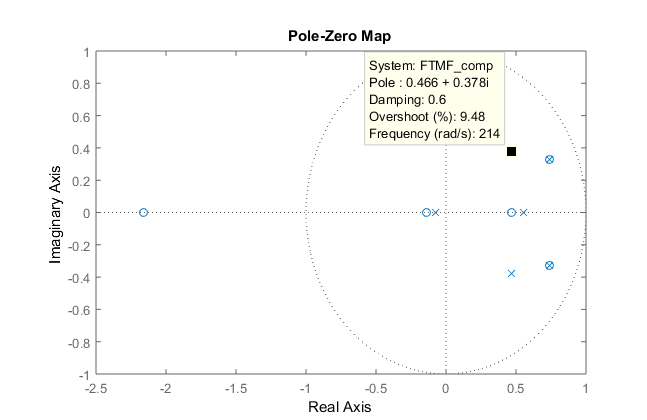
\includegraphics[scale=0.9]{./img/verificPolosFTMFcomp.png}
	\label{fig:verificPolosFTMFcomp}
	\legend{Software: MATLAB}
\end{figure}

\pagebreak

\section{\textbf{Teste e Resultado.}}

\subsection{Teste utilizando Simulink.}
Como a ação de controle do microcontrolador é limitada pelas características do PWM, sendo que esse apenas pode gerar uma ação de controle que vai de zero até a tensão do nível lógico do microcontrolador, é preciso verificar se a ação de controle não vai sofrer uma saturação.
Como o sinal de estímulo é um degrau que vai de 1 V até 1.5 V, na rampa de descida a ação de controle não pode ter o módulo da sua amplitude maior que 1.5 V, do contrário irá saturar 0 V.
Por meio da ferramenta Simulink embutida no MATLAB, é possível fazer a verificação da amplitude da ação de controle. Na \autoref{fig:simulink_FTMF} é apresentado o esquemático utilizado para a simulação no Simulink:

\begin{figure}[htb!]
	\centering
	\caption{Esquemático do sistema de controle em malha fechada.}
	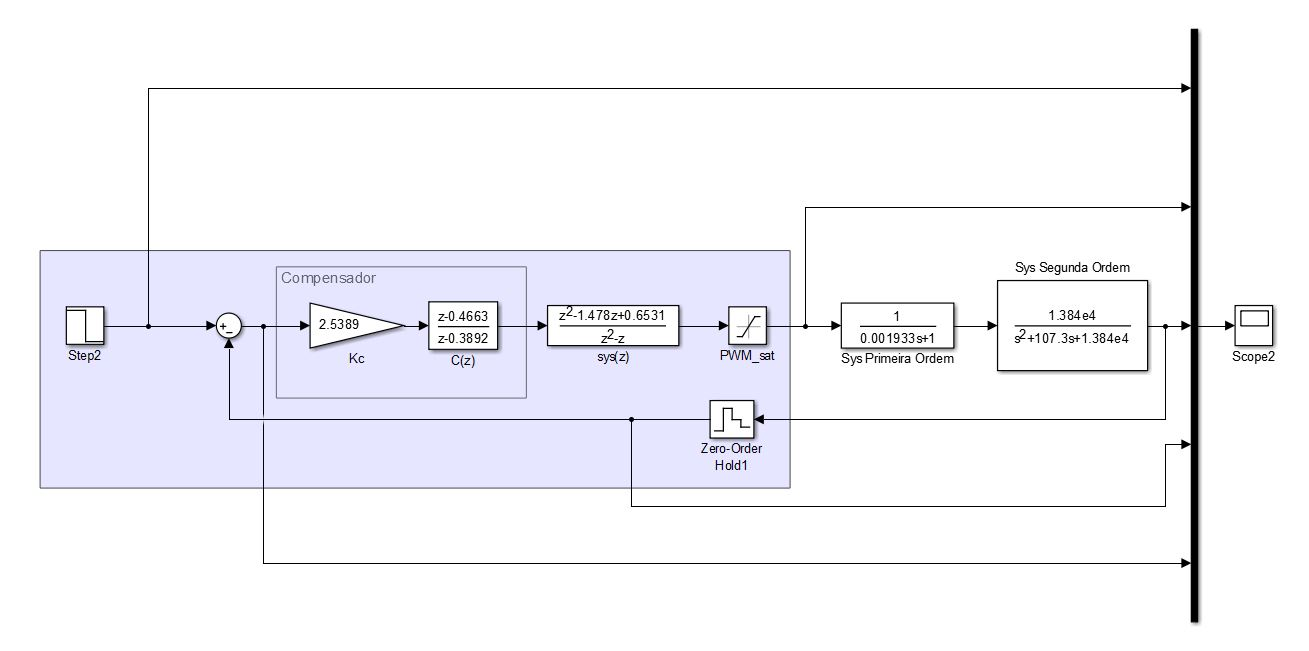
\includegraphics[scale=0.40]{./img/simulink_FTMF.JPG}
	\label{fig:simulink_FTMF}
	\legend{Software: MATLAB}
\end{figure}

Medindo a saída do controlador é possível verificar que a máxima variação da amplitude da ação de controle é de 1.269 V. Logo para o degrau subindo de 1 V para 1.5 V a máxima ação de controle é $1+1.269 = 2.269$ V e para a descida do degrau a mínima ação de controle é $1.5-1.269 = 0.231$ V. Logo não ocorrerá saturação da ação de controle (\autoref{fig:step_CtrlActionSimulink}).

\begin{figure}[htb!]
	\centering
	\caption{Verificação da amplitude da ação de controle - Simulink.}
	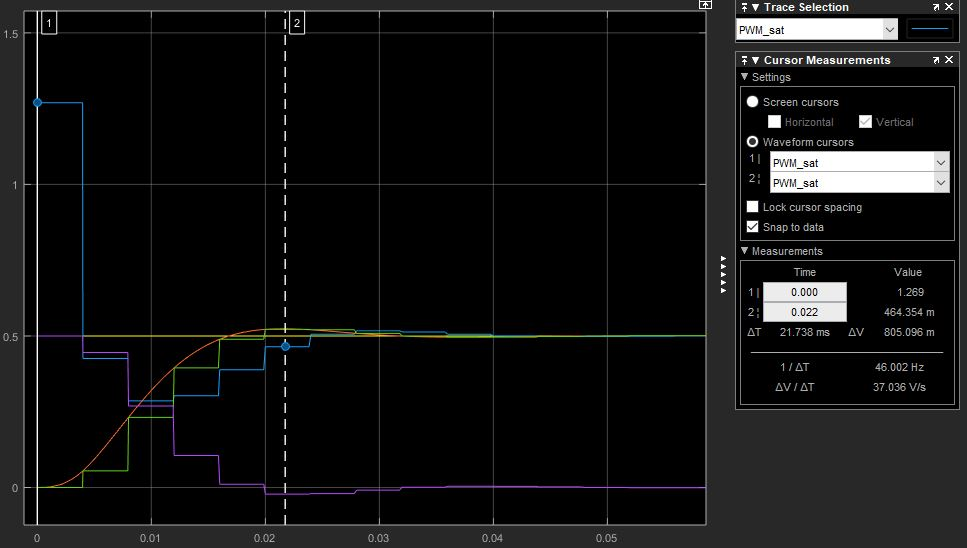
\includegraphics[scale=0.4]{./img/step_CtrlActionSimulink.JPG}
	\label{fig:step_CtrlActionSimulink}
	\legend{Software: MATLAB}
\end{figure}

\pagebreak

\subsection{Teste utilizando Equações Recursivas.}

Como a compensador será implementado no microcontrolador em forma de equações de diferenças, as funções de transferência desenvolvidas anteriormente devem ser expressas na forma de equações de diferenças para serem resolvidas de forma recursiva.
Para testar essas equações de diferenças antes de implementa-las no microcontrolador, o script MATLAB apresentado no \autoref{app:scriptEqRecursivas} é capaz de operar recursivamente as equações diferenças de cada bloco apresentadas abaixo:
$$P1(z)*P2(z)*Z(z)*C(z)*G(z)$$
Equação e diferenças do sistema de polos e zeros acrescentados á planta:
$$P1(z)*P2(z)*Z(z) = \frac{Y_{ZP}(z)}{X_{ZP}(z)} = \frac{z^2 - 1.478 z + 0.6531}{z^2-z}$$
$$Y_{ZP}(z)(z^2-z) = X_{ZP}(z)(z^2 - 1.478 z + 0.6531)$$
$$y_{ZP}[n+2]-y_{ZP}[n+1] = x_{ZP}[n+2] - 1.478x_{ZP}[n+1] + 0.6531x_{ZP}[n]$$
$$y_{ZP}[n] = x_{ZP}[n] - 1.478x_{ZP}[n-1] + 0.6531x_{ZP}[n-2]+y_{ZP}[n-1]$$
Equação de diferenças do compensador:
$$C(z) = \frac{Y_{C}(z)}{X_{C}(z)} = 2.5389 * \frac{z - 0.4663}{z - 0.3892}$$ 
$$Y_{C}(z)(z - 0.3892) = X_{C}(z)(2.5389*(z - 0.4663))$$
$$y_{C}[n+1] - 0.3892y_{C}[n] = 2.5389x_{C}[n+1]-(2.5389*0.4663)x_{C}[n]$$
$$y_C[n] =  2.5389*x_C[n] - 1.1839*x_C[n-1] + 0.3892*y_C[n-1];$$
Equação de diferenças da planta:
$$G(z) = \frac{Y_{G}(z)}{X_{G}(z)} = \frac{0.04241z^2 + 0.09738z + 0.01247}{z^3 - 1.607z^2 + 0.8424z - 0.08366}$$
$$Y_{G}(z)(z^3 - 1.607z^2 + 0.8424z - 0.08366) = X_{G}(z)(0.04241z^2 + 0.09738z + 0.01247)$$
$$y_{G}[n+3] - 1.607y_{G}[n+2] + 0.8424y_{G}[n+1] - 0.08366y_{G}[n] =$$ 
$$=0.04241x_{G}[n+2] + 0.09738x_{G}[n+1]  + 0.01247x_{G}[n] $$
$$y_{G}[n] = 0.04241x_{G}[n-1] + 0.09738x_{G}[n-2]  + 0.01247x_{G}[n-3] +$$ 
$$+1.607y_{G}[n-1] - 0.8424y_{G}[n-2] + 0.08366y_{G}[n-3]  $$

O script MATLAB apresentado no \autoref{app:scriptEqRecursivas} também mostra como essas equações de diferenças foram conectadas para serem resolvidas recursivamente. 

\pagebreak

Com o uso do script MATLAB contido no \autoref{app:scriptEqRecursivas}, a \autoref{fig:EqRecursiva_testeMatlab} foi traçada mostrando que as equações recursivas operadas iterativamente apresentaram o mesmo valor da resposta ao degrau do sistema FTMF(z) compensado.
Os pontos em forma de "x" vermelho representam o sinal de erro. Os pontos em forma de "*" representam a saída do sistema da equações recursivas e o traçado azul representa resultado do comando \textit{step()} do MATLAB para o sistema FTMF(z) compensado.

\begin{figure}[htb!]
	\centering
	\caption{Verificação da resposta ao degrau da equação recursiva.}
	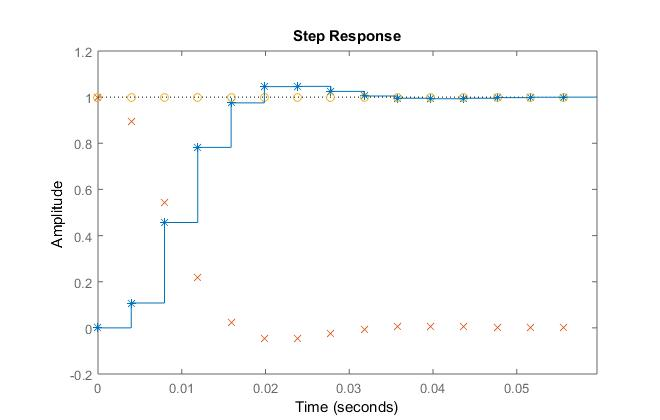
\includegraphics[scale=0.7]{./img/EqRecursiva_testeMatlab.jpg}
	\label{fig:EqRecursiva_testeMatlab}
	\legend{Software: MATLAB}
\end{figure}

\pagebreak

\subsection{Teste experimental.}

Fazendo a leitura via UART é possível verificar que o sinal com o compensador está apresentando a resposta esperada com valores próximos aos resultados da simulação.

\begin{figure}[htb!]
	\centering
	\caption{Verificação da resposta ao degrau da equação recursiva.}
	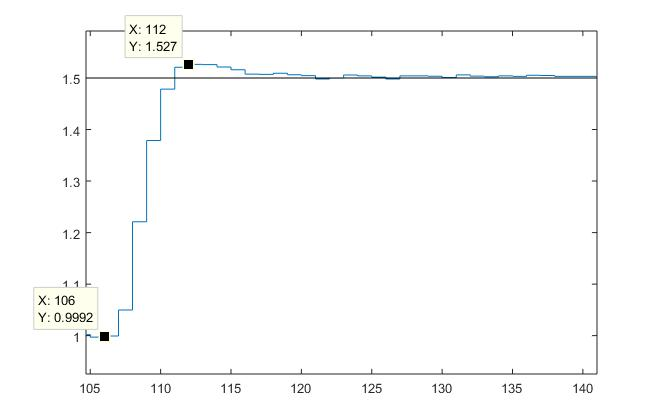
\includegraphics[scale=0.7]{./img/stepExperMatlab_comp.jpg}
	\label{fig:stepExperMatlab_comp}
	\legend{Software: MATLAB}
\end{figure}
Lembrando que o resultado da simulação apresentou  $M_p = 4.69\%$ e  $T_p/T = 6$ (\autoref{fig:stepComp}), o sobressinal e o tempo de pico tomando como base a \autoref{fig:stepExperMatlab_comp} é:
$$
	100\% => 0.500
$$
$$
	M_p\% + 100\%=> 1.527 - 0.999 = 0.528 => 105.6\%
$$
$$
	M_p\% = 5.6\%
$$
$$
T_p/T = 112 - 106 = 6
$$

\pagebreak

Por meio de um osciloscópio digital é possível verificar com uma taxa de amostragem muito maior que a \autoref{fig:stepExperMatlab_comp} o comportamento da saída. 
É verificado o sobressinal $M_p$ na \autoref{fig:mp_compensado}:

\begin{figure}[htb!]
\begin{center}
	\caption{Verificação da resposta ao degrau da equação recursiva.}
	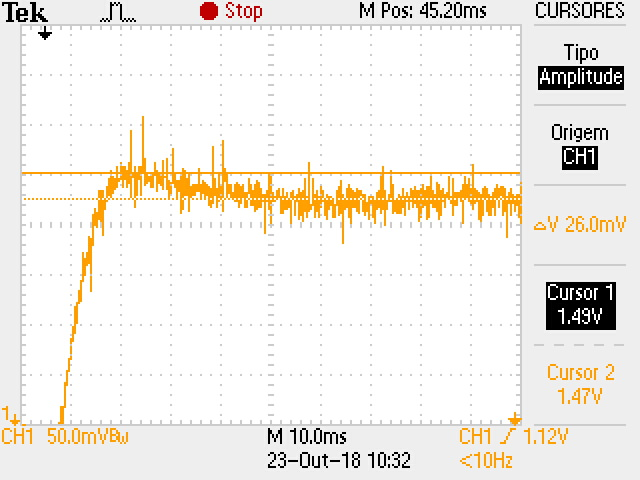
\includegraphics[scale=1.4]{./img/mp_compensado.JPG}
	\label{fig:mp_compensado}
	\legend{Osciloscópio Tektronics Tds1002c}
\end{center}
\end{figure}

Apesar do ruído presente na \autoref{fig:mp_compensado}, por meio dos cursores é possível estimar um valor aproximado de $M_p \simeq 5.2\%$:

$$
	100\% => 0.500 V
$$
$$
	M_p\% => 0.026 V\%
$$
$$
	M_p\% = 5.2\%
$$

\pagebreak

Levando em consideração a simulação (\autoref{fig:stepComp}), o sobressinal se mostra menor que $5\%$ e o tempo de acomodação $T_s (5\%)$ acontece antes do tempo de pico $T_p$. 
Porém a resultado prático apresentou um valor de sobressinal $M_p$ um pouco maior que $5\%$: $M_p = 5.6\%$ segundo a \autoref{fig:stepExperMatlab_comp} e $M_p \simeq 5.2\%$  segundo a \autoref{fig:mp_compensado}.
Considerando a situação da simulação, onde o tempo de acomodação acontece antes do tempo de sobressinal, o $T_s (5\%)$ acontece aproximadamente aos $15.6 ms$ como pode ser verificado na \autoref{fig:ts5_compensado}.

\begin{figure}[htb!]
	\centering
	\caption{Verificação da resposta ao degrau da equação recursiva.}
	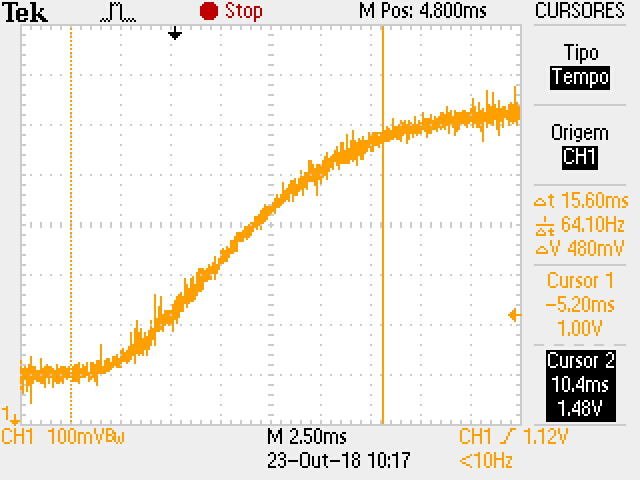
\includegraphics[scale=1]{./img/ts5_compensado.JPG}
	\label{fig:ts5_compensado}
	\legend{Osciloscópio Tektronics Tds1002c}
\end{figure}

Por outro lado considerando a situação do teste experimental onde o sobressinal é praticamente igual a $5\%$ como verificado na \autoref{fig:stepExperMatlab_comp} e \autoref{fig:mp_compensado}, tempo de sobressinal $T_p$ é praticamente igual ao tempo $T_s (5\%)$. 
Logo na \autoref{fig:tp_compensado} é verificado $T_s (5\%) \simeq  T_p \simeq 21.6 ms$.

\begin{figure}[htb!]
	\centering
	\caption{Verificação da resposta ao degrau da equação recursiva.}
	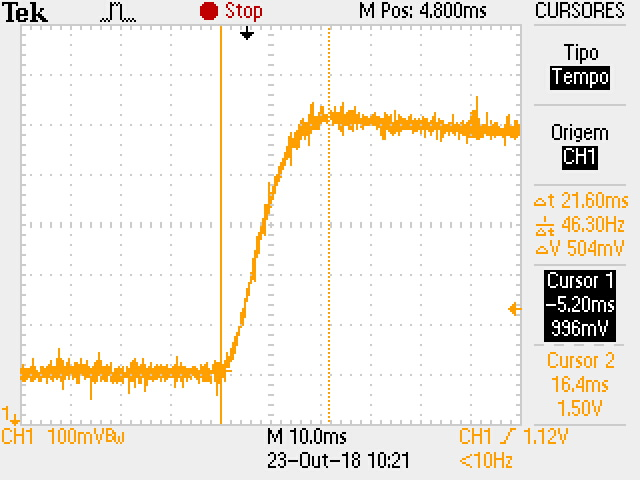
\includegraphics[scale=1]{./img/tp_compensado.JPG}
	\label{fig:tp_compensado}
	\legend{Osciloscópio Tektronics Tds1002c}
\end{figure}

Porém para ambas as situações o requisito de projeto para o $T_s (5\%)$ foi atingido (metade do $T_s (5\%)=47 ms$ da resposta ao degrau da planta: $T_s (5\%)/2=23.5 ms$.

\pagebreak

A \autoref{tab:tabelaResultados} apresenta um comparativo dos resultados obtidos. São apresentados os casos experimentais onde se considera o $T_{s5\%}$ acontecendo antes e depois do $T_p$, onde $M_p$ é menor ou mair que $5\%$.
\begin{table}[htbp]
\caption{Tabela comparativa de resultados.}
\begin{center}
\begin{tabular}{|l|l|l|l|l|l|}
\hline
 & Simulação & Experimental & Experimental & Requisitos & Planta (FTMA) \\ \hline
$M_p$ (\%) & $4.69$ & se $M_p<5\%$ & $5.2$ & $10.0$ & $20.0$ \\ \hline
$T_{s5\%}$ (ms) & $15.4$ & $15.6$ & $21.6$ & $23.4$ & $46.7$ \\ \hline
\end{tabular}
\end{center}
\label{tab:tabelaResultados}
\end{table}

Também foi medido o tempo de processamento, do inicio da requisição do valor no ADC até a atualização do PWM. A \autoref{fig:tempoDeProcessamento} mostra o valor do tempo de processamento de cada amostra da \autoref{fig:amostras_tempoDeProcessamento}. É possível notar que o tempo de processamento se manteve constante com valor em torno de $243 \mu s$.

\begin{figure}[htb!]
	\centering
	\caption{Tempo de processamento de cada amostra da \autoref{fig:amostras_tempoDeProcessamento}.}
	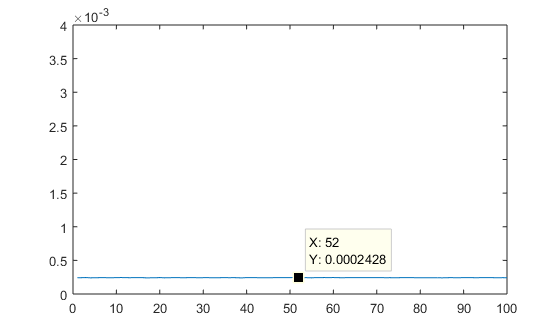
\includegraphics[scale=0.6]{./img/tempoDeProcessamento.png}
	\label{fig:tempoDeProcessamento}
	\legend{Software: MATLAB}
\end{figure}

\begin{figure}[htb!]
	\centering
	\caption{Amostras de cada tempo coletado e apresentado na \autoref{fig:tempoDeProcessamento}.}
	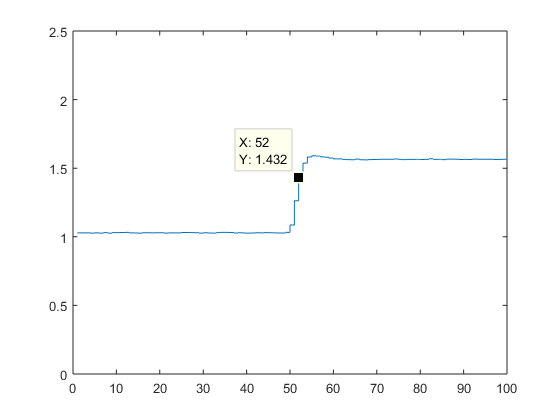
\includegraphics[scale=0.6]{./img/amostras_tempoDeProcessamento.png}
	\label{fig:amostras_tempoDeProcessamento}
	\legend{Software: MATLAB}
\end{figure}



\pagebreak

\section{\textbf{Conclusão}}
 
Com a atividade descrita ao longo desse relatório foi possível verificar a possibilidade de uma implementação de um sistema de controle para plantas analógicas com uso de um processador digital.
Que apesar da limitação devido ao tempo de processamento, que ocasiona uma taxa de amostragem finita, esses sistemas digitais podem interagir com o mundo do tempo contínuo afim de controlar uma gama de sistemas analógicos que possuem constantes de tempo relativamente grande em comparação ao período de amostragem.
Para isso basta que o sistema digital possa ser interfaceado com o mundo analógico, por meio de conversores analógicos digitais (ADCs) e moduladores de largura de pulso (PWMs) em intervalos de tempo espaçados pelo período de amostragem.

Nessa atividade foi constatado como as constantes de tempo e dinâmica de uma planta podem ser extraídas tanto de forma experimental quanto analítica e como essas formas de analise fornecem resultados parecidos mas não idênticos.
E tendo o conhecimento das constantes de tempo e dinâmica da planta também foi verificado como é possível fazer a compensação da resposta da planta por meio de um sistema digital modelado no plano Z.
Durante a fase de projeto o sistema digital apresentou uma vantagem em relação a projeto de compensadores analógicos: A possibilidade de mudar o \textit{software} que modela o sistema sem alterar o \textit{hardware}.

Apesar de não serem idênticos, os resultados práticos se aproximaram satisfatoriamente das simulações e os requisitos de projeto foram atendidos.
E dessa forma foi evidenciando a possibilidade que os processadores digitais fornecem aos projetistas de sistema de controle, de modelar sistemas de ordem e complexidade elevada sem a necessidade de um grande volume de \textit{hardware}.
%
%
%
%
\pagebreak

% ----------------------------------------------------------
% ELEMENTOS PÓS-TEXTUAIS
% ----------------------------------------------------------
\postextual

% ---
% Título e resumo em língua estrangeira
% ---

% ----------------------------------------------------------
% Referências bibliográficas
% ----------------------------------------------------------
\bibliography{bib_eletronic.eng}

% ----------------------------------------------------------
% Glossário
% ----------------------------------------------------------
%
% Há diversas soluções prontas para glossário em LaTeX. 
% Consulte o manual do abnTeX2 para obter sugestões.
%
%\glossary

% ----------------------------------------------------------
% Apêndices
% ----------------------------------------------------------

% ---
% Inicia os apêndices
% ---
\begin{apendicesenv}
	
	% Imprime uma página indicando o início dos apêndices
	\partapendices

\chapter{Script MATLAB para o cálculo do somatório dos ângulos}
% ----------------------------------------------------------
	\label{app:scriptCalcAng}
\lstset{language=MATLAB}
\begin{lstlisting}
%% calculador de angulo: polos
deltaPolos_img = zeros(1, length(Gz_polos)); 
deltaPolos_real = deltaPolos_img;
angPolos = deltaPolos_img; 
angPolosGrau = deltaPolos_img;

for i=1:length(Gz_polos)
    if z_real < real(Gz_polos(i))
        deltaPolos_real(i) = real(Gz_polos(i)) - z_real;        
        if z_imag < imag(Gz_polos(i))
            deltaPolos_img(i) = imag(Gz_polos(i)) - z_imag;
            angPolos(i) = pi + atan(deltaPolos_img(i)/deltaPolos_real(i));
        else
            deltaPolos_img(i) = z_imag - imag(Gz_polos(i));
            angPolos(i) = pi - atan(deltaPolos_img(i)/deltaPolos_real(i));
        end           
    else
        deltaPolos_real(i) = z_real - real(Gz_polos(i));          
        if z_imag < imag(Gz_polos(i))
            deltaPolos_img(i) = imag(Gz_polos(i)) - z_imag;
            angPolos(i) = 2*pi - atan(deltaPolos_img(i)/deltaPolos_real(i));
        else
            deltaPolos_img(i) = z_imag - imag(Gz_polos(i));
            angPolos(i) = atan(deltaPolos_img(i)/deltaPolos_real(i));
        end                
    end 
    angPolosGrau(i) = (180*angPolos(i))/pi;
end
\end{lstlisting}

\lstset{language=MATLAB}
\begin{lstlisting}
%% calculador de angulo: zeros
deltaZeros_img = zeros(1, length(Gz_zeros)); 
deltaZeros_real = deltaZeros_img;
angZeros = deltaZeros_img; 
angZerosGrau = deltaZeros_img;

for i=1:length(Gz_zeros)
    if z_real < real(Gz_zeros(i))
        deltaZeros_real(i) = real(Gz_zeros(i)) - z_real;        
        if z_imag < imag(Gz_zeros(i))
            deltaZeros_img(i) = imag(Gz_zeros(i)) - z_imag;
            angZeros(i) = pi + atan(deltaZeros_img(i)/deltaZeros_real(i));
        else
            deltaZeros_img(i) = z_imag - imag(Gz_zeros(i));
            angZeros(i) = pi - atan(deltaZeros_img(i)/deltaZeros_real(i));
        end           
    else
        deltaZeros_real(i) = z_real - real(Gz_zeros(i));          
        if z_imag < imag(Gz_zeros(i))
            deltaZeros_img(i) = imag(Gz_zeros(i)) - z_imag;
            angZeros(i) = 2*pi - atan(deltaZeros_img(i)/deltaZeros_real(i));
        else
            deltaZeros_img(i) = z_imag - imag(Gz_zeros(i));
            angZeros(i) = atan(deltaZeros_img(i)/deltaZeros_real(i));
        end                
    end 
    angZerosGrau(i) = (180*angZeros(i))/pi;
end
\end{lstlisting}

\pagebreak

\chapter{Script MATLAB para teste das equações recursivas}
% ----------------------------------------------------------
\label{app:scriptEqRecursivas}

\lstset{language=MATLAB}
\begin{lstlisting}
%% Equacao recursiva: Coeficientes Fixos
plotSize=50; kT = T*(0:plotSize-1);
c=zeros(1, plotSize); r=zeros(1, plotSize); e=zeros(1, plotSize);
y_Gz=zeros(1, plotSize); x_Gz=zeros(1, plotSize);
y_Cz=zeros(1, plotSize); x_Cz=zeros(1, plotSize);
y_ZPz=zeros(1, plotSize); x_ZPz=zeros(1, plotSize);
r(1:plotSize)=1;

i=1;      
    x_Cz(i)=y_Gz(i);   
    y_Cz(i) =  2.5389*x_Cz(i);   
    x_ZPz(i)=y_Cz(i);     
    y_ZPz(i) = x_ZPz(i);
    c(i) = y_ZPz(i);
    e(i) = r(i)-c(i);    
    x_Gz(i) = e(i);

i=2;   
    y_Gz(i) =  0.0424*x_Gz(i-1) + 1.6065*y_Gz(i-1);       
    x_Cz(i)=y_Gz(i);   
    y_Cz(i) =  2.5389*x_Cz(i) - 1.1839*x_Cz(i-1) + 0.3892*y_Cz(i-1);   
    x_ZPz(i)=y_Cz(i);     
    y_ZPz(i) = x_ZPz(i) - 1.4780*x_ZPz(i-1) + y_ZPz(i-1);
    c(i) = y_ZPz(i);
    e(i) = r(i)-c(i);    
    x_Gz(i) = e(i);

i=3;
    y_Gz(i) =  0.0424*x_Gz(i-1) + 0.0974*x_Gz(i-2) + 1.6065*y_Gz(i-1) - 0.8424*y_Gz(i-2);       
    x_Cz(i)=y_Gz(i);   
    y_Cz(i) =  2.5389*x_Cz(i) - 1.1839*x_Cz(i-1) + 0.3892*y_Cz(i-1);   
    x_ZPz(i)=y_Cz(i);     
    y_ZPz(i) = x_ZPz(i) - 1.4780*x_ZPz(i-1) + 0.6531*x_ZPz(i-2) + y_ZPz(i-1);
    c(i) = y_ZPz(i);
    e(i) = r(i)-c(i);    
    x_Gz(i) = e(i);
    
for i=4:plotSize   
    y_Gz(i) =  0.0424*x_Gz(i-1) + 0.0974*x_Gz(i-2) + 0.0125*x_Gz(i-3) + 1.6065*y_Gz(i-1) - 0.8424*y_Gz(i-2) + 0.0837*y_Gz(i-3);       
    x_Cz(i)=y_Gz(i);   
    y_Cz(i) =  2.5389*x_Cz(i) - 1.1839*x_Cz(i-1) + 0.3892*y_Cz(i-1);    
    x_ZPz(i)=y_Cz(i);     
    y_ZPz(i) = x_ZPz(i) - 1.4780*x_ZPz(i-1) + 0.6531*x_ZPz(i-2) + y_ZPz(i-1);
    c(i) = y_ZPz(i);
    e(i) = r(i)-c(i);    
    x_Gz(i) = e(i);
end

plot(kT, c, '*')
hold on
plot(kT, e, 'x')
plot(kT, r, 'o')
step(FTMF_comp);
xlim([0 T*plotSize]); ylim([-3 3]);
hold off
\end{lstlisting}

\pagebreak

\chapter{Firmware Completo do Sistema de Controle}
% ----------------------------------------------------------
	\label{app:FirmwareCompleto}
	
	\lstset{language=C}
	\begin{lstlisting}
#include "project.h"

// -----------------------------------------------------------------------------
#define OFF_COMMAND 0x00
#define FULL_COMMAND  0xff

#define ENABLE_COMMAND 0b00000001 
#define RESET_COMMAND  0b00000010

#define CLOSELOOP_COMMAND 0b00000100
#define COMP_ON_COMMAND   0b00001000
#define ZPSYS_ON_COMMAND  0b00010000
uint32 streamSys_status;

uint8 uartOut_array[6];
uint16 adcBuffer, outputBuffer;
uint32 cycleCounter;
float32 adcBufferFloat, erroBuffer, inputBuffer;
float32 Gc_inputBuffer[2], Gc_outputBuffer[2], Gc_K = 2.5389, Gc_beta=-0.3892, Gc_alpha=-0.4663;
float32 sys_inputBuffer[3], sys_outputBuffer[3];

// -----------------------------------------------------------------------------
// State Machine ---------------------------------------------------------------
void exit_state_process();//0
void start_state_process();//1
void standby_state_process();//2
void scanOn_state_process();//3
void scanOff_state_process();//4
void sampler_state_process();//5
void closeLoop_state_process();//6
void openLoop_state_process();//7
void compOn_state_process();//8
void compOff_state_process();//9
void zpsysOn_state_process();//10
void zpsysOff_state_process();//11
void ctrlOn_state_process();//12
void ctrlOff_state_process();//13

//Estado comum a todas as máquinas de estado:
#define EXIT_STATE 0
#define START_STATE 1
#define STANDBY_STATE 2
#define SCANON_STATE 3
#define SCANOFF_STATE 4
#define SAMPLER_STATE 5
#define CLOSELOOP_STATE 6
#define OPENLOOP_STATE 7
#define COMPON_STATE 8
#define COMPOFF_STATE 9
#define ZPSYSON_STATE 10
#define ZPSYSOFF_STATE 11
#define CTRLON_STATE 12
#define CTRLOFF_STATE 13

void (*main_state_table[])()=
{
    exit_state_process,//0
    start_state_process,//1
    standby_state_process,//2
    scanOn_state_process,//3
    scanOff_state_process,//4
    sampler_state_process,//5
    closeLoop_state_process,//6
    openLoop_state_process,//7
    compOn_state_process,//8
    compOff_state_process,//9
    zpsysOn_state_process,//10
    zpsysOff_state_process,//11
    ctrlOn_state_process,//12
    ctrlOff_state_process//13
};

volatile int main_state;

CY_ISR(samplerInterrupt_handler)
{	
    main_state =  SAMPLER_STATE;
}

CY_ISR(RxInterrupt_1)
{	
    main_state = UART_1_GetChar();
}

CY_ISR(stepInterrupt_handler)
{	
    //inputBuffer = 0.666;
    inputBuffer = 0.335;
    //inputBuffer = 1;
    //inputBuffer = 0.420;
}

CY_ISR(zeroInterrupt_handler)
{	
    //inputBuffer = 0.333;
    inputBuffer = 0.2225;
    //inputBuffer = 0;
    //inputBuffer = 0.150;
}

int main(void)
{
    CyGlobalIntEnable; /* Enable global interrupts. */

    UART_1_Start();
    isr_Rx_1_StartEx(RxInterrupt_1);
     
    isr_SamplerStateSig_StartEx(samplerInterrupt_handler);
    isr_SamplerStateSig_Disable();
    
    isr_stepSig_StartEx(stepInterrupt_handler);
    isr_zeroSig_StartEx(zeroInterrupt_handler);
    
    Control_Reg_1_Write(OFF_COMMAND);   
    
    while(1)
    {
        main_state = START_STATE;
        while(main_state)
        {       
            main_state_table[main_state]();
        }
    }
}

void exit_state_process()//0
{
   isr_SamplerStateSig_Disable();
}

void start_state_process()//1
{
    streamSys_status = streamSys_status&(~CLOSELOOP_COMMAND); 
    streamSys_status = streamSys_status&(~COMP_ON_COMMAND);
    streamSys_status = streamSys_status&(~ZPSYS_ON_COMMAND); 
    
    streamSys_status = streamSys_status|CLOSELOOP_COMMAND;
    streamSys_status = streamSys_status|COMP_ON_COMMAND;
    streamSys_status = streamSys_status|ZPSYS_ON_COMMAND;  
    
    Control_Reg_1_Write(OFF_COMMAND);
    
    Timer_1_Start();
}

void standby_state_process()//2
{
    
}

void scanOn_state_process()//3
{
    main_state = STANDBY_STATE;
    
    isr_SamplerStateSig_Enable();
    
    isr_stepSig_Enable();
    isr_zeroSig_Enable();
    
    ADC_DelSig_Start();

    PWM_Start();
    PWM_WriteCompare(10);
    
    Control_Reg_1_Write(ENABLE_COMMAND);
}

void scanOff_state_process()//4
{
    main_state = STANDBY_STATE;
    
    isr_SamplerStateSig_Disable();
    
    ADC_DelSig_Stop();
    
    PWM_Stop();
    
    Control_Reg_1_Write(OFF_COMMAND);   
}

#define CLOSELOOP_COMMAND 0b00000100
#define COMP_ON_COMMAND  0b00001000
#define ZPSYS_ON_COMMAND 0b00010000

void sampler_state_process()//5
{
    main_state = STANDBY_STATE;
 
    //*******************************************************************
    //Counter Start:
    Timer_1_WriteCounter(1000000);
    //*******************************************************************
       
    //-------------------------------------------------------------------
    adcBuffer = ADC_DelSig_Read16(); 
    adcBufferFloat=((float32)adcBuffer)/(0xffff);    
    
    //-------------------------------------------------------------------
    //Opened-Loop or Closed-Loop:
    if(streamSys_status&CLOSELOOP_COMMAND)
        erroBuffer = inputBuffer - adcBufferFloat;//Closed-Loop        
    else
        erroBuffer = inputBuffer;
    //-------------------------------------------------------------------

    Gc_inputBuffer[0] = erroBuffer; 
    
    //-------------------------------------------------------------------
    //Compensator ON or OFF:
    if(streamSys_status&COMP_ON_COMMAND)
        Gc_outputBuffer[0] = Gc_K*Gc_inputBuffer[0] + Gc_K*Gc_alpha*Gc_inputBuffer[1] - Gc_beta*Gc_outputBuffer[1];//ON         
    else
        Gc_outputBuffer[0] = Gc_inputBuffer[0];//OFF         
    //-------------------------------------------------------------------    
    sys_inputBuffer[0] = Gc_outputBuffer[0]; 
    //-------------------------------------------------------------------
    if(streamSys_status&ZPSYS_ON_COMMAND)
        sys_outputBuffer[0] =  sys_inputBuffer[0] - 1.478*sys_inputBuffer[1] + 0.6531*sys_inputBuffer[2] + sys_outputBuffer[1];//ON        
    else
        sys_outputBuffer[0] = sys_inputBuffer[0];//OFF                        
    //-------------------------------------------------------------------
  
    outputBuffer = (uint16)(sys_outputBuffer[0]*0xffff);   
    PWM_WriteCompare(outputBuffer);
    
    //*******************************************************************
    //Counter End:
    cycleCounter = Timer_1_ReadCounter(); 
    //*******************************************************************  
    
    Gc_inputBuffer[1] = Gc_inputBuffer[0];
    Gc_outputBuffer[1] = Gc_outputBuffer[0];
    
    sys_inputBuffer[2] = sys_inputBuffer[1];
    sys_outputBuffer[2] = sys_outputBuffer[1];  
    sys_inputBuffer[1] = sys_inputBuffer[0];
    sys_outputBuffer[1] = sys_outputBuffer[0];
     
    //-------------------------------------------------------------------
    adcBuffer = (uint16)(adcBufferFloat*0xffff);
    
    uartOut_array[0]=adcBuffer;
    uartOut_array[1]=adcBuffer>>8;
    
    uartOut_array[2]=cycleCounter;
    uartOut_array[3]=cycleCounter>>8;
    uartOut_array[4]=cycleCounter>>16;
    uartOut_array[5]=cycleCounter>>24;
    
    UART_1_PutArray(uartOut_array, 6);
}

void closeLoop_state_process()//6
{
    main_state = STANDBY_STATE;
    streamSys_status = streamSys_status|CLOSELOOP_COMMAND;   
}

void openLoop_state_process()//7
{
    main_state = STANDBY_STATE;
    streamSys_status = streamSys_status&(~CLOSELOOP_COMMAND);    
}

void compOn_state_process()//8
{
    main_state = STANDBY_STATE;
    streamSys_status = streamSys_status|COMP_ON_COMMAND; 
}

void compOff_state_process()//9
{
    main_state = STANDBY_STATE;
    streamSys_status = streamSys_status&(~COMP_ON_COMMAND); 
}

void zpsysOn_state_process()//10
{
    main_state = STANDBY_STATE;
    streamSys_status = streamSys_status|ZPSYS_ON_COMMAND; 
}

void zpsysOff_state_process()//11
{
    main_state = STANDBY_STATE;
    streamSys_status = streamSys_status&(~ZPSYS_ON_COMMAND);   
}

void ctrlOn_state_process()//12
{
    main_state = STANDBY_STATE;
    streamSys_status = streamSys_status|CLOSELOOP_COMMAND;
    streamSys_status = streamSys_status|COMP_ON_COMMAND;
    streamSys_status = streamSys_status|ZPSYS_ON_COMMAND;     
}

void ctrlOff_state_process()//13
{
    main_state = STANDBY_STATE;
    streamSys_status = streamSys_status&(~CLOSELOOP_COMMAND); 
    streamSys_status = streamSys_status&(~COMP_ON_COMMAND);
    streamSys_status = streamSys_status&(~ZPSYS_ON_COMMAND); 
}
	\end{lstlisting}
	\pagebreak
	
\end{apendicesenv}
% ---

\pagebreak
\end{document}


